\section{Phát hiện Vật thể (Object Detection)}
\label{sec:object_detection}

Nếu phân loại ảnh là bước đầu tiên để một cỗ máy "nhận biết" thế giới, thì phát hiện vật thể là bước nhảy vọt thực sự hướng tới sự "thấu hiểu". Bài toán không còn dừng lại ở việc gán một nhãn chung cho toàn bộ bức ảnh, mà đòi hỏi mô hình phải trả lời hai câu hỏi cùng một lúc: \textbf{"Có những vật thể gì trong ảnh?" (Phân loại)} và \textbf{"Chúng đang ở đâu?" (Định vị)}.

Đầu ra của một mô hình phát hiện vật thể không phải là một nhãn duy nhất, mà là một danh sách các đối tượng được tìm thấy. Mỗi đối tượng được biểu diễn bởi:
\begin{itemize}
	\item Một \textbf{khung hộp bao (bounding box)}, thường được định nghĩa bởi tọa độ của góc trên bên trái và góc dưới bên phải $(x_{min}, y_{min}, x_{max}, y_{max})$.
	\item Một \textbf{nhãn lớp (class label)} cho đối tượng bên trong hộp (ví dụ: "chó", "mèo", "ô tô").
	\item Một \textbf{điểm số tự tin (confidence score)}, cho biết mức độ chắc chắn của mô hình về dự đoán của nó.
\end{itemize}

Lịch sử phát triển của các thuật toán phát hiện vật thể trong kỷ nguyên học sâu là một cuộc chạy đua hấp dẫn giữa hai trường phái chính:
\begin{enumerate}
	\item \textbf{Các bộ phát hiện hai giai đoạn (Two-stage detectors):} Hoạt động theo nguyên lý "nhìn kỹ". Giai đoạn đầu tiên đề xuất một tập hợp các vùng có khả năng chứa vật thể (region proposals), và giai đoạn thứ hai phân loại và tinh chỉnh các vùng đó. Chúng thường có độ chính xác cao hơn.
	\item \textbf{Các bộ phát hiện một giai đoạn (One-stage detectors):} Hoạt động theo nguyên lý "nhìn một lần". Chúng dự đoán trực tiếp vị trí và lớp của các vật thể từ ảnh đầu vào chỉ trong một lượt duy nhất, không có bước đề xuất vùng riêng biệt. Chúng thường nhanh hơn rất nhiều.
\end{enumerate}
Trong phần này, chúng ta sẽ lần theo dấu chân của cả hai trường phái này, từ những ý tưởng sơ khai đến các kiến trúc state-of-the-art ngày nay.

\subsection{Kỷ nguyên CNN: Từ R-CNN đến YOLO và SSD}
\label{subsec:cnn_based_detectors}

Sự thành công của AlexNet trong phân loại ảnh năm 2012 đã mở ra một câu hỏi cấp thiết: làm thế nào để áp dụng sức mạnh trích xuất đặc trưng của CNN cho bài toán phát hiện vật thể phức tạp hơn?

\subsubsection{Họ R-CNN: Cách tiếp cận Hai giai đoạn}
\label{subsubsec:r_cnn_family}

\paragraph{R-CNN (2014):}
\textbf{Regions with CNN features (R-CNN)} \cite{Girshick2014} là mô hình tiên phong đưa sức mạnh của CNN vào bài toán phát hiện vật thể, đánh dấu sự chuyển dịch dứt khoát từ các đặc trưng thủ công (HOG, DPM) sang biểu diễn học sâu. Ý tưởng trung tâm rất đơn giản: \textit{nếu CNN có thể nhận dạng vật thể khi được đưa toàn bộ bức ảnh, tại sao không ``cắt'' các vùng có khả năng chứa vật thể ra rồi đưa từng vùng vào CNN?}

\textbf{Bước 1 — Sinh vùng đề xuất với Selective Search.}
Trước khi CNN xử lý bất cứ điều gì, R-CNN cần biết \textit{nên nhìn vào đâu}. Nhiệm vụ này được giao cho thuật toán \textbf{Selective Search}: thay vì quét toàn bộ ảnh theo kiểu cửa sổ trượt (sliding window) --- cách tiếp cận cổ điển nhưng tốn kém --- Selective Search phân tích ảnh theo màu sắc, kết cấu, kích thước và tính liên tục để đề xuất khoảng \textbf{2000 vùng} (region proposals) có khả năng cao chứa vật thể.

Mỗi vùng đề xuất $R_i$ là một hình chữ nhật trên ảnh gốc. Selective Search không học từ dữ liệu --- nó hoạt động thuần túy bằng heuristic --- nhưng đảm bảo recall cao: hầu hết các vật thể thật sự trong ảnh đều được bao phủ bởi ít nhất một trong 2000 vùng đó.

\begin{center}
	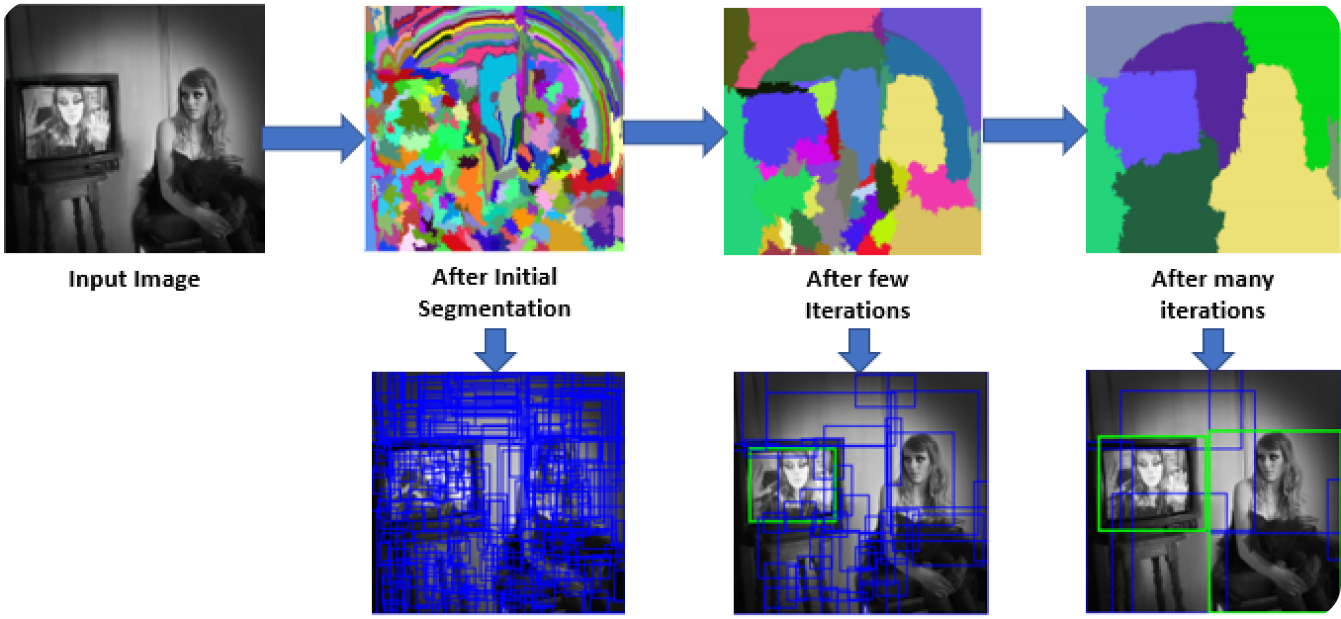
\includegraphics[width=1.0\textwidth]
	{images/selective_search.png}
	\captionof{figure}{Cách Selective Search hoạt động: thuật toán phân cụm dựa trên màu sắc, kết cấu và kích thước để đề xuất các vùng có khả năng chứa vật thể.}
	\label{fig:rcnn_pipeline}
\end{center}

\textbf{Bước 2 — Trích xuất đặc trưng bằng CNN.}
Mỗi trong 2000 vùng được cắt ra từ ảnh gốc, sau đó \textit{warp} (co giãn cưỡng bức) về kích thước cố định $227 \times 227$ pixel --- đây là kích thước đầu vào của AlexNet, backbone mà R-CNN sử dụng. Từng vùng riêng lẻ được đưa qua CNN và thu về một vector đặc trưng $\mathbf{f}_i \in \mathbb{R}^{4096}$. Đây là bước tốn kém nhất: với 2000 vùng, mô hình phải chạy \textbf{2000 lần forward pass} qua CNN cho mỗi bức ảnh, khiến thời gian inference lên tới $\sim 47$ giây/ảnh.

Thao tác warp làm mất tỷ lệ khung hình ban đầu của vùng đề xuất --- một con người cao gầy sẽ bị kéo thành béo, một chiếc xe ô tô nằm ngang bị bóp méo thành hình vuông --- nhưng đây là sự đánh đổi chấp nhận được để CNN có đầu vào kích thước nhất quán.

\textbf{Bước 3 — Phân loại bằng SVM.}
Sau khi có vector đặc trưng $\mathbf{f}_i$, R-CNN \textit{không} dùng lớp softmax của CNN để phân loại. Thay vào đó, nó huấn luyện một bộ \textbf{SVM tuyến tính riêng biệt cho mỗi lớp vật thể}. Với bài toán PASCAL VOC 20 lớp cần 20 SVM; với 200 lớp ImageNet Detection cần 200 SVM. Lý do dùng SVM thay vì softmax là vì tại thời điểm 2014, SVM huấn luyện trên đặc trưng CNN cho độ chính xác cao hơn --- một dấu hiệu cho thấy fine-tuning CNN trực tiếp cho detection chưa được tối ưu hoàn toàn.

\begin{mdframed}[style=infobox]
\textbf{Intersection over Union (IoU) và Non-Maximum Suppression (NMS)}

Hai khái niệm này xuất hiện ở khắp mọi bộ phát hiện vật thể, và R-CNN là nơi chúng được hệ thống hóa rõ ràng lần đầu.

\textbf{IoU} đo mức độ chồng lấp giữa bounding box dự đoán $A$ và ground-truth $B$:
\[
\text{IoU}(A, B) = \frac{\text{Area}(A \cap B)}{\text{Area}(A \cup B)}
\]
IoU = 1 nghĩa là hai box hoàn toàn trùng nhau; IoU = 0 nghĩa là không có điểm chung. Trong R-CNN, một vùng đề xuất được coi là \textit{positive} (chứa vật thể) nếu IoU với ground-truth $\geq 0.5$, và \textit{negative} (nền) nếu IoU $< 0.3$. Các vùng có IoU nằm trong khoảng $[0.3, 0.5)$ bị bỏ qua khi huấn luyện để tạo margin phân cách rõ ràng.

\textbf{NMS} giải quyết tình trạng nhiều vùng cùng phát hiện một vật thể. Thuật toán hoạt động theo nguyên tắc greedy: (1) chọn box có score cao nhất làm đại diện, (2) loại bỏ tất cả box khác có IoU với box đó vượt ngưỡng $\tau$ (thường 0.5), (3) lặp lại cho đến khi không còn box nào. Kết quả là mỗi vật thể chỉ còn một bounding box tốt nhất.
\end{mdframed}

\textbf{Bước 4 — Tinh chỉnh vị trí bằng hồi quy bounding box.}
SVM cho biết \textit{vùng đó chứa gì}, nhưng vùng đề xuất từ Selective Search thường không khớp hoàn hảo với vật thể thực sự. Bước cuối cùng là dùng một mô hình hồi quy tuyến tính để tinh chỉnh tọa độ. Thay vì dự đoán tọa độ tuyệt đối, mô hình học các \textit{offset tương đối} so với vùng đề xuất ban đầu $(x_a, y_a, w_a, h_a)$:
\[
t_x = \frac{x^* - x_a}{w_a}, \quad t_y = \frac{y^* - y_a}{h_a}, \quad t_w = \log \frac{w^*}{w_a}, \quad t_h = \log \frac{h^*}{h_a}
\]
trong đó $(x^*, y^*, w^*, h^*)$ là ground-truth. Hàm log cho $t_w, t_h$ giúp chuẩn hóa bài toán: thay vì học tỷ lệ nhân (multiplicative scale), mô hình chỉ cần học phép cộng trên log-scale --- dễ hội tụ hơn nhiều và cân bằng gradient giữa vật thể nhỏ và lớn.

\begin{center}
	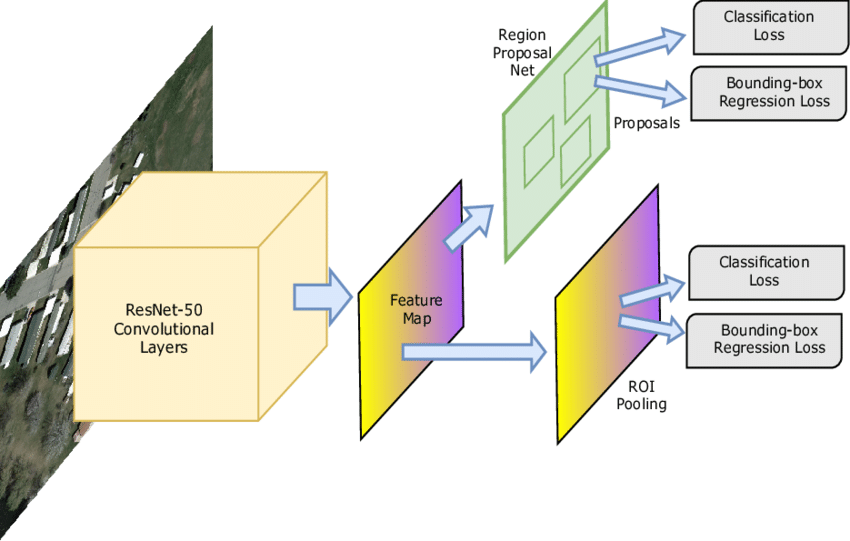
\includegraphics[width=1.0\textwidth]
	{images/rcnn_pipeline_diagram.png}
	\captionof{figure}{Pipeline của R-CNN gồm 4 bước: Selective Search đề xuất $\sim$2000 vùng, mỗi vùng được warp và đưa qua CNN riêng lẻ, SVM phân loại từng vùng, và bộ hồi quy tinh chỉnh bounding box.}
	\label{fig:rcnn_pipeline_diagram}
\end{center}

\textbf{Huấn luyện — Ba giai đoạn rời rạc.}
R-CNN không thể được huấn luyện end-to-end trong một bước. Quá trình gồm ba giai đoạn hoàn toàn tách biệt: (1) \textbf{Pre-train CNN} trên ImageNet để có backbone mạnh; (2) \textbf{Fine-tune CNN} trên dữ liệu detection với các vùng có IoU $\geq 0.5$ là positive và còn lại là negative; (3) \textbf{Train SVM và bộ hồi quy} riêng lẻ trên các đặc trưng đã được lưu vào đĩa từ bước trước.

Sự tách biệt này có một hệ quả kiến trúc quan trọng: gradient từ SVM và bộ hồi quy \textit{không} lan truyền ngược về CNN. CNN không biết rằng đặc trưng nó tạo ra cuối cùng được dùng để phân loại và định vị --- nó chỉ được fine-tune cho mục đích phân loại thông thường. Đây là một điểm yếu cơ bản của toàn bộ pipeline.

Ngoài ra, một kỹ thuật quan trọng giúp cải thiện SVM là \textbf{Hard Negative Mining}: sau mỗi vòng huấn luyện, chọn lọc những negative samples mà mô hình đang phân loại sai (những vùng nền bị nhầm là vật thể) và thêm chúng vào tập huấn luyện lần sau. Điều này tránh để mô hình lãng phí dung lượng trên những ví dụ nền quá dễ.

\textbf{Tổng kết.}
R-CNN tăng mAP trên PASCAL VOC 2012 từ 40.9\% (DPM) lên \textbf{53.3\%} --- một cú nhảy vọt chứng minh sức mạnh của CNN cho detection. Tuy nhiên, mô hình có ba hạn chế cấu trúc nghiêm trọng: (i) \textbf{chậm} ($\sim$47 giây/ảnh khi test, $\sim$84 giờ để train trên VOC) vì phải chạy CNN 2000 lần; (ii) \textbf{không end-to-end}, huấn luyện rời rạc không tối ưu joint, tốn bộ nhớ đĩa để lưu feature trung gian; (iii) \textbf{warping distortion} gây biến dạng hình học ảnh hưởng đến localization.

Những hạn chế này chính là bản thiết kế cho Fast R-CNN: \textit{thay vì chạy CNN trên từng vùng, tại sao không chạy CNN một lần duy nhất trên toàn ảnh rồi chia sẻ kết quả?}

\paragraph{Fast R-CNN (2015):}
Vấn đề của R-CNN nằm ở một nghịch lý: để phân tích 2000 vùng đề xuất, nó phải chạy CNN 2000 lần --- dù phần lớn các vùng đó chồng chéo lên nhau và chia sẻ nhiều pixel chung. Năm 2015, Ross Girshick đề xuất \textbf{Fast R-CNN} \cite{Girshick2015} với một câu hỏi đơn giản: \textit{tại sao không chạy CNN một lần duy nhất trên toàn ảnh, rồi trích xuất đặc trưng của từng vùng từ kết quả đó?}

\begin{center}
	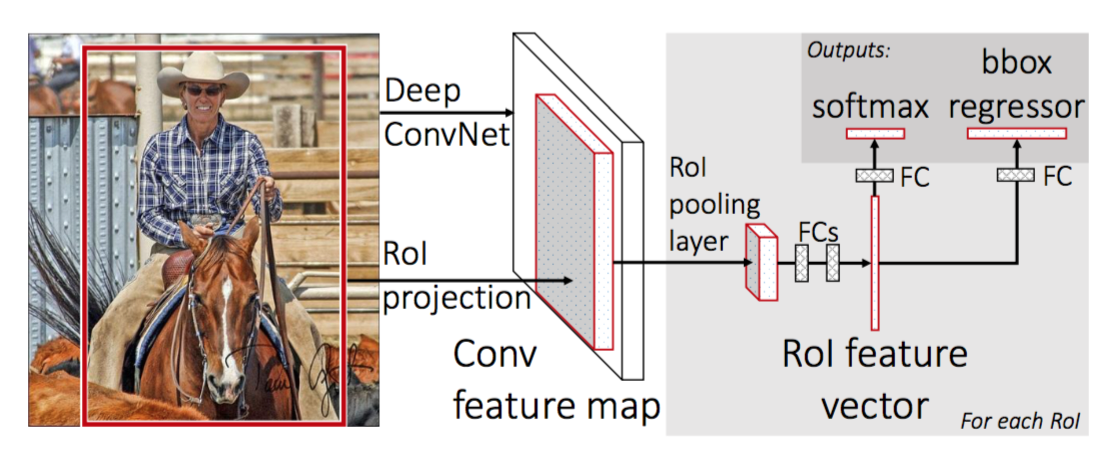
\includegraphics[width=0.95\textwidth]{images/fast_rcnn_architecture.png}
	\captionof{figure}{Kiến trúc Fast R-CNN. Thay vì CNN chạy trên từng vùng riêng lẻ như R-CNN, toàn bộ ảnh được đưa qua CNN một lần duy nhất để tạo ra feature map chung. Mỗi vùng đề xuất sau đó được trích xuất từ feature map này thông qua RoI Pooling.}
	\label{fig:fast_rcnn_arch}
\end{center}

\textbf{Ý tưởng cốt lõi — Chia sẻ feature map.}
Fast R-CNN chỉ chạy CNN \textit{một lần} trên toàn bộ ảnh đầu vào $I$, tạo ra một feature map chung:
\[
F = \text{CNN}(I) \in \mathbb{R}^{C \times H' \times W'}
\]
Tất cả 2000 vùng đề xuất (vẫn được tạo bởi Selective Search) sau đó được \textit{chiếu lên} feature map $F$ thay vì chạy CNN riêng từng vùng. Trong R-CNN, một pixel thuộc vùng chồng lấp giữa nhiều proposal có thể được CNN xử lý hàng trăm lần; trong Fast R-CNN, mỗi pixel chỉ đi qua CNN \textbf{đúng một lần}. Điều này giảm độ phức tạp từ $O(N \cdot \text{CNN})$ xuống $O(\text{CNN}) + O(N)$ --- một bậc giảm theo hệ số $N \approx 2000$.

\textbf{RoI Projection — Ánh xạ vùng lên feature map.}
Một vùng đề xuất $R_i = (x_1, y_1, x_2, y_2)$ trên ảnh gốc được chiếu xuống feature map theo tỷ lệ stride $s$ của CNN:
\[
R_i' = \left(\left\lfloor\frac{x_1}{s}\right\rfloor,\ \left\lfloor\frac{y_1}{s}\right\rfloor,\ \left\lfloor\frac{x_2}{s}\right\rfloor,\ \left\lfloor\frac{y_2}{s}\right\rfloor\right)
\]
Phép làm tròn tọa độ ở bước này gây ra sai số lượng tử hóa nhỏ --- đây chính là điểm yếu sẽ được Mask R-CNN khắc phục sau này bằng RoIAlign.

\textbf{RoI Pooling — Chuẩn hóa kích thước đặc trưng.}
Sau khi chiếu, mỗi vùng $R_i'$ trên feature map có kích thước khác nhau. Fast R-CNN dùng \textbf{RoI Pooling} để đưa tất cả về kích thước cố định $H_f \times W_f$ (thường là $7 \times 7$):

\begin{enumerate}
	\item Chia vùng $R_i'$ thành lưới $H_f \times W_f$ ô (bins) có kích thước xấp xỉ bằng nhau.
	\item Áp dụng max-pooling trong mỗi bin: $f_i^{(u,v)} = \max_{(x,y) \in \text{bin}(u,v)} F(x,y)$
	\item Flatten kết quả thành vector đặc trưng $\mathbf{f}_i \in \mathbb{R}^{C \cdot H_f \cdot W_f}$
\end{enumerate}

Kỹ thuật này cho phép Fast R-CNN xử lý các vùng đề xuất có kích thước tùy ý mà không cần warping như R-CNN --- không còn biến dạng hình học.

\begin{center}
	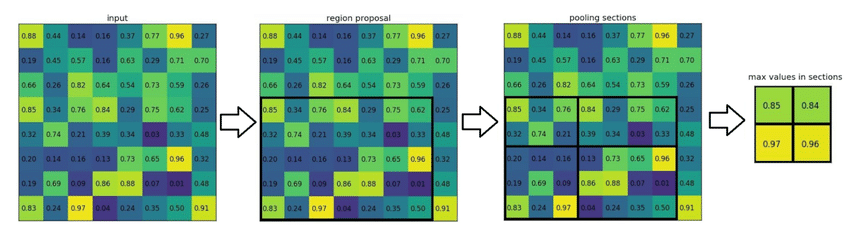
\includegraphics[width=0.8\textwidth]{images/roi_pooling_diagram.png}
	\captionof{figure}{Minh họa RoI Pooling: một vùng đề xuất kích thước bất kỳ trên feature map được chia thành lưới $H_f \times W_f$ cố định, max-pooling áp dụng trên từng ô.}
	\label{fig:roi_pooling}
\end{center}

\begin{center}
	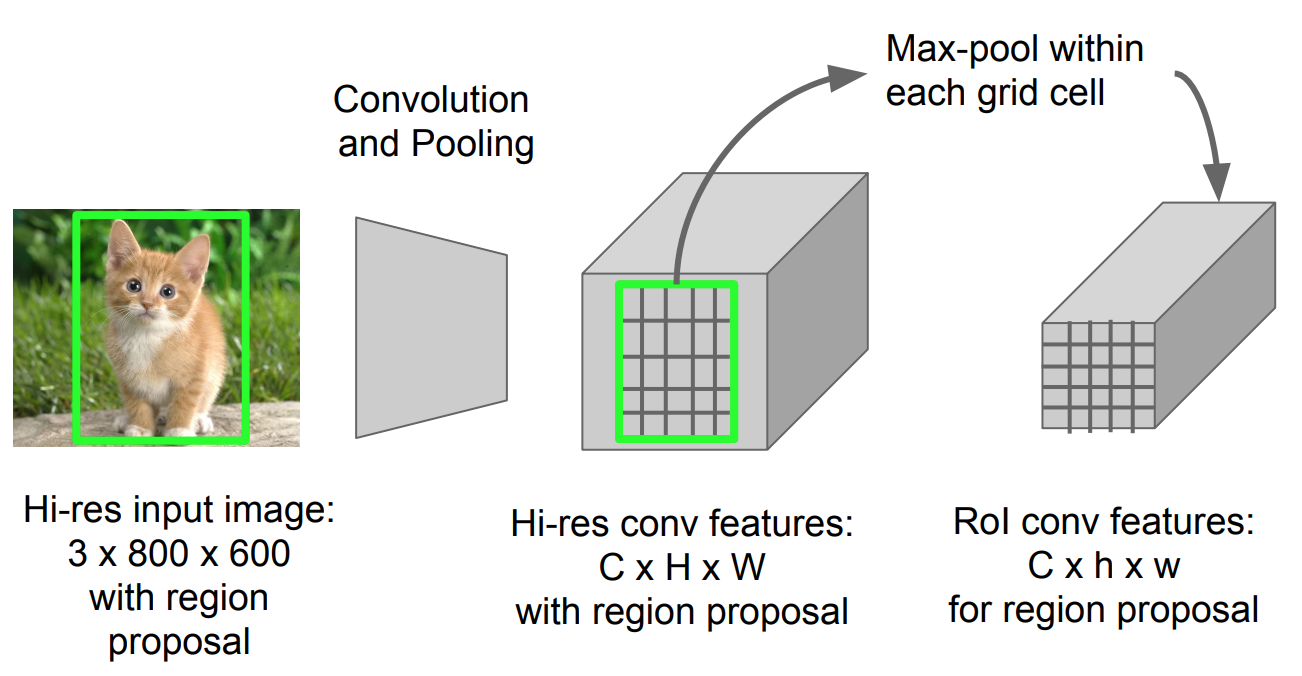
\includegraphics[width=0.75\textwidth]{images/roi_pooling_lilian.png}
	\captionof{figure}{Ví dụ cụ thể RoI Pooling: vùng $5 \times 7$ trên feature map được chia thành lưới $2 \times 2$, mỗi ô lấy giá trị max. Kết quả luôn là tensor $2 \times 2$ bất kể kích thước đầu vào.}
	\label{fig:roi_pooling_detail}
\end{center}

\textbf{Đầu phân loại và hồi quy (Head Network).}
Vector đặc trưng $\mathbf{f}_i$ sau RoI Pooling được đưa qua các fully-connected layers rồi tách thành \textit{hai nhánh song song}:
\begin{itemize}
	\item \textbf{Nhánh phân loại:} $p_i = \text{softmax}(W_c \mathbf{f}_i) \in \mathbb{R}^{K+1}$ — xác suất cho $K$ lớp vật thể cộng với lớp nền. Không cần SVM nữa!
	\item \textbf{Nhánh hồi quy:} $t_i = W_r \mathbf{f}_i \in \mathbb{R}^{4K}$ — offsets bounding box cho từng lớp.
\end{itemize}

\textbf{Hàm mất mát multi-task.}
Fast R-CNN được huấn luyện end-to-end với một hàm mất mát duy nhất tối ưu cả phân loại lẫn định vị cùng lúc:
\[
\mathcal{L} = L_{\text{cls}}(p_i,\, c_i^*) + \lambda \cdot \mathbf{1}[c_i^* \geq 1] \cdot L_{\text{reg}}(t_i,\, t_i^*)
\]

Trong đó $c_i^*$ là nhãn ground-truth và $\mathbf{1}[c_i^* \geq 1]$ đảm bảo loss hồi quy chỉ tính khi đó là vật thể thật (không tính với nền). Thành phần phân loại dùng cross-entropy chuẩn:
\[
L_{\text{cls}} = -\log p_i[c_i^*]
\]

Còn thành phần hồi quy dùng \textbf{Smooth L1 loss} thay vì MSE:
\[
\text{Smooth}_{L_1}(x) = \begin{cases} 0.5x^2 & \text{nếu } |x| < 1 \\ |x| - 0.5 & \text{ngược lại} \end{cases}
\]

\begin{center}
	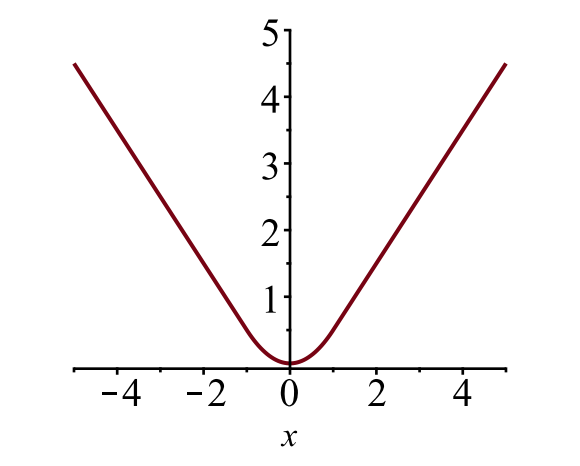
\includegraphics[width=0.60\textwidth]{images/smooth_l1_loss.png}
	\captionof{figure}{So sánh hình dạng của Smooth L1, L1 và L2 loss. Smooth L1 hành xử như L2 (quadratic) khi sai số nhỏ --- ổn định gradient --- và như L1 (linear) khi sai số lớn --- robust với outlier.}
	\label{fig:smooth_l1}
\end{center}

Lý do dùng Smooth L1: L2 loss phạt rất mạnh các outlier (bounding box dự đoán sai nhiều), khiến gradient bùng nổ; trong khi L1 thuần túy có gradient không liên tục tại 0 gây mất ổn định. Smooth L1 kết hợp ưu điểm của cả hai: mượt mà gần 0 và chịu đựng tốt outlier.

\textbf{Huấn luyện end-to-end và tăng tốc đáng kể.}
Khác với R-CNN cần 3 giai đoạn riêng biệt, Fast R-CNN được huấn luyện \textit{trong một bước duy nhất}: gradient từ loss lan truyền ngược qua head network, qua RoI Pooling, qua feature map, và về tận CNN backbone. Điều này có nghĩa là CNN được fine-tune trực tiếp cho mục tiêu detection --- không còn rào cản giữa classifier và feature extractor. Kết quả:

\begin{itemize}
	\item Thời gian train giảm từ 84 giờ (R-CNN) xuống còn \textbf{9.5 giờ} trên VOC 2007
	\item Thời gian test giảm từ 47 giây/ảnh xuống còn \textbf{0.32 giây/ảnh} (không tính Selective Search)
	\item mAP trên VOC 2007 tăng từ 66.0\% (R-CNN) lên \textbf{70.0\%}
\end{itemize}

\begin{mdframed}[style=infobox]
\textbf{Bottleneck cuối cùng: Selective Search}

Với Fast R-CNN, thời gian inference trên GPU chỉ còn 0.32 giây/ảnh cho phần CNN. Tuy nhiên, \textit{Selective Search} vẫn chạy trên CPU và chiếm khoảng \textbf{2 giây/ảnh} --- gấp 6 lần phần CNN! Nói cách khác, bottleneck không còn là mạng nơ-ron mà là bước tạo proposal ngoài mô hình. Đây chính là lý do Faster R-CNN ra đời: thay Selective Search bằng một mạng nơ-ron có thể học được và chạy trên GPU.
\end{mdframed}

Đây chính là động lực dẫn đến Faster R-CNN với Region Proposal Network.


\paragraph{Faster R-CNN (2016):}
Khi Fast R-CNN ra đời, bottleneck không còn là CNN nữa --- mà là \textbf{Selective Search} đang chạy trên CPU, chiếm $\sim$2 giây/ảnh trong khi toàn bộ phần CNN chỉ mất 0.32 giây. Câu hỏi đặt ra: \textit{nếu ta có thể học cách phát hiện vật thể bằng mạng nơ-ron, tại sao không học luôn cả cách đề xuất vùng?} Đây chính là đột phá của \textbf{Faster R-CNN} \cite{Ren2015} — thay thế hoàn toàn Selective Search bằng một mạng nơ-ron có thể học được, chạy trên GPU và chia sẻ feature với detector chính.

\begin{center}
	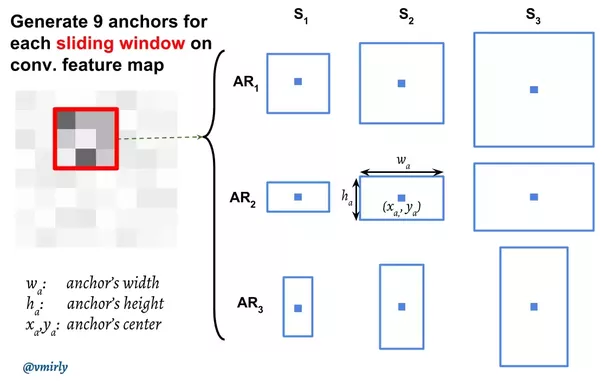
\includegraphics[width=0.90\textwidth]{images/faster_rcnn_overview.png}
	\captionof{figure}{Các anchor box được đặt tại mỗi vị trí trên feature map với nhiều kích thước và tỷ lệ khung hình khác nhau. RPN học dự đoán: anchor nào chứa vật thể (objectness score) và cần dịch chuyển bao nhiêu để khớp với vật thể thực.}
	\label{fig:faster_rcnn_overview}
\end{center}

\textbf{Kiến trúc tổng thể — Ba thành phần chia sẻ feature.}
Faster R-CNN gồm ba thành phần chính, cùng dùng chung một feature map $F$:
\begin{enumerate}
	\item \textbf{Backbone CNN} (thường là VGG-16 hoặc ResNet): chạy \textit{một lần} trên toàn ảnh, tạo ra feature map $F \in \mathbb{R}^{C \times H' \times W'}$.
	\item \textbf{Region Proposal Network (RPN)}: nhận $F$ làm đầu vào, đề xuất các vùng có khả năng chứa vật thể.
	\item \textbf{Fast R-CNN detection head}: nhận $F$ và các vùng đề xuất từ RPN, phân loại và tinh chỉnh bounding box.
\end{enumerate}

Điểm mấu chốt: RPN và detection head \textit{dùng chung backbone} --- không có phép tính nào bị lặp lại. Điều này đồng nghĩa với việc đề xuất vùng giờ đây gần như miễn phí về mặt tính toán.

\textbf{Region Proposal Network (RPN) — Học cách nhìn.}
RPN là một \textbf{Fully Convolutional Network} nhỏ trượt trên feature map $F$ bằng cửa sổ $3 \times 3$. Tại mỗi vị trí $(i,j)$ trên feature map, RPN đặt $k = 9$ \textbf{anchor box} --- các hộp tham chiếu với 3 kích thước (128, 256, 512 pixel) và 3 tỷ lệ khung hình (1:1, 1:2, 2:1). Với feature map $H' \times W'$, tổng số anchor trong toàn ảnh là $H' \times W' \times 9$ --- thường khoảng 20.000 anchor cho ảnh $600 \times 1000$ pixel.

\begin{center}
	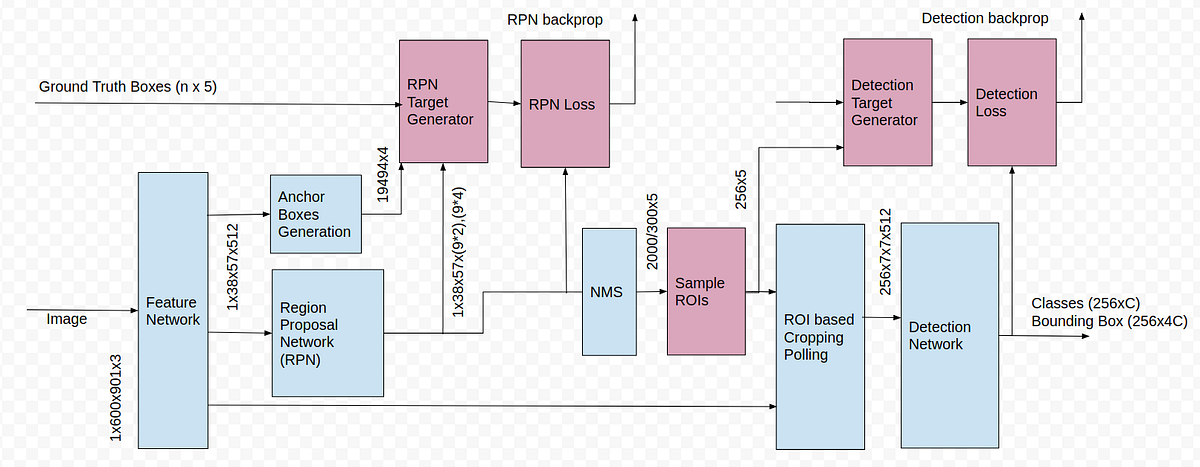
\includegraphics[width=0.95\textwidth]{images/rpn_anchors.png}
	\captionof{figure}{Kiến trúc tổng quan Faster R-CNN: backbone CNN tạo ra feature map dùng chung cho cả RPN (sinh vùng đề xuất) và Fast R-CNN head (phân loại và tinh chỉnh box). Toàn bộ pipeline chạy trên GPU, không còn phụ thuộc Selective Search.}
	\label{fig:rpn_anchors}
\end{center}

Với mỗi anchor, RPN dự đoán hai thứ song song:
\begin{itemize}
	\item \textbf{Objectness score} $p_i \in [0,1]$: xác suất anchor chứa vật thể (foreground) hay chỉ là nền (background).
	\item \textbf{Bounding box offset} $(t_x, t_y, t_w, t_h)$: độ lệch cần thiết để biến anchor thành proposal khớp với vật thể hơn:
\end{itemize}
\[
t_x = \frac{x^* - x_a}{w_a},\quad t_y = \frac{y^* - y_a}{h_a},\quad t_w = \log\frac{w^*}{w_a},\quad t_h = \log\frac{h^*}{h_a}
\]

\textbf{Gán nhãn anchor trong huấn luyện.}
Để huấn luyện RPN, mỗi anchor cần được gán nhãn \textit{positive} hoặc \textit{negative} dựa trên IoU với ground-truth:
\begin{itemize}
	\item \textbf{Positive}: anchor có IoU $\geq 0.7$ với bất kỳ ground-truth nào, \textit{hoặc} anchor có IoU cao nhất với một ground-truth (đảm bảo mỗi ground-truth luôn có ít nhất một anchor positive).
	\item \textbf{Negative}: anchor có IoU $< 0.3$ với \textit{mọi} ground-truth.
	\item \textbf{Bỏ qua}: anchor nằm trong khoảng $[0.3, 0.7)$ --- vùng mơ hồ, không dùng để tính loss tránh nhiễu gradient.
\end{itemize}

Vì số anchor negative (nền) nhiều hơn positive gấp hàng chục lần, RPN dùng \textbf{mini-batch sampling}: mỗi ảnh lấy ngẫu nhiên 256 anchor với tỷ lệ positive:negative tối đa là 1:1 (nếu không đủ positive thì lấy thêm negative bù vào).

\textbf{Hàm mất mát của RPN.}
RPN được tối ưu với hàm mất mát multi-task:
\[
\mathcal{L}_{\text{RPN}} = \frac{1}{N_{\text{cls}}} \sum_i L_{\text{cls}}(p_i,\, p_i^*) + \lambda \cdot \frac{1}{N_{\text{reg}}} \sum_i p_i^* \cdot L_{\text{reg}}(t_i,\, t_i^*)
\]

Trong đó $p_i^*$ là nhãn ground-truth (1 nếu positive, 0 nếu negative), đóng vai trò mask để chỉ tính regression loss cho các anchor positive. $N_{\text{cls}}$ và $N_{\text{reg}}$ là các hệ số chuẩn hóa giúp cân bằng hai thành phần loss.

\textbf{Từ anchor đến proposal — Lọc qua NMS.}
Sau khi RPN chạy, mỗi anchor được biến thành một proposal bằng cách áp dụng offset dự đoán. Tiếp theo:
\begin{enumerate}
	\item Loại bỏ các proposal vượt ra ngoài biên ảnh.
	\item Sắp xếp theo objectness score, giữ top-$N$ cao nhất (thường $N = 6000$ khi train, 300 khi test).
	\item Áp dụng NMS với ngưỡng IoU = 0.7 để loại proposal trùng lặp.
	\item Kết quả: $\sim$2000 proposal khi train, $\sim$300 khi test.
\end{enumerate}
Những proposal này thay thế hoàn toàn output của Selective Search --- và được tạo ra \textit{trong vài mili giây} trên GPU thay vì 2 giây trên CPU.

\textbf{Giai đoạn detection — Tái sử dụng feature map.}
Các proposal từ RPN được đưa vào Fast R-CNN head \textit{trên cùng feature map $F$}: RoI Pooling trích xuất đặc trưng $7 \times 7$ cho từng proposal, sau đó head network phân loại lớp vật thể và tinh chỉnh lần cuối tọa độ bounding box. Loss toàn bộ mạng là tổng của RPN loss và detector loss:
\[
\mathcal{L} = \mathcal{L}_{\text{RPN}} + \mathcal{L}_{\text{detector}}
\]

\textbf{Chiến lược huấn luyện.}
Faster R-CNN có hai cách huấn luyện: (1) \textbf{Alternating training} --- luân phiên train RPN rồi detector, lặp lại 4 lần --- đây là cách trong bài báo gốc; (2) \textbf{Approximate joint training} --- tối ưu đồng thời toàn bộ mạng trong một bước, nhanh hơn $\sim$1.5 lần và cho kết quả tương đương, được dùng phổ biến trong thực tế.

\begin{mdframed}[style=infobox]
\textbf{Kết quả và tầm quan trọng}

Faster R-CNN đạt \textbf{73.2\% mAP} trên PASCAL VOC 2007 với VGG-16, vượt Fast R-CNN (70.0\%). Quan trọng hơn, tốc độ inference giảm từ $\sim$2.3 giây/ảnh (Fast R-CNN + Selective Search) xuống còn \textbf{0.2 giây/ảnh} --- gần 10 lần nhanh hơn. Đây là lần đầu tiên một two-stage detector đạt tốc độ gần real-time.

Faster R-CNN thiết lập kiến trúc chuẩn cho mọi two-stage detector sau này: \textbf{Backbone → RPN → RoI Pooling → Head}. Các mô hình như Mask R-CNN, Cascade R-CNN, hay DetectoRS đều xây dựng trực tiếp trên nền tảng này.
\end{mdframed}

Đây là bước chuyển quyết định từ \textbf{pipeline rời rạc} (Selective Search ngoài mạng) sang \textbf{hệ thống học thống nhất hoàn toàn} --- đặt nền tảng vững chắc cho toàn bộ thế hệ detector hiện đại.


\paragraph{Mask R-CNN (2017):}
Nếu Faster R-CNN trả lời câu hỏi \textit{"Vật thể ở đâu?"} bằng một bounding box, thì \textbf{Mask R-CNN} \cite{He2017} của Kaiming He và cộng sự (Facebook AI Research) đặt ra câu hỏi tham vọng hơn: \textit{"Chính xác pixel nào thuộc về vật thể đó?"} Đây là bài toán \textbf{instance segmentation} --- không chỉ khoanh vùng vật thể bằng hộp chữ nhật mà còn vẽ ra đường viền chính xác từng pixel, phân biệt được từng cá thể ngay cả khi chúng chồng chéo nhau.

\begin{center}
	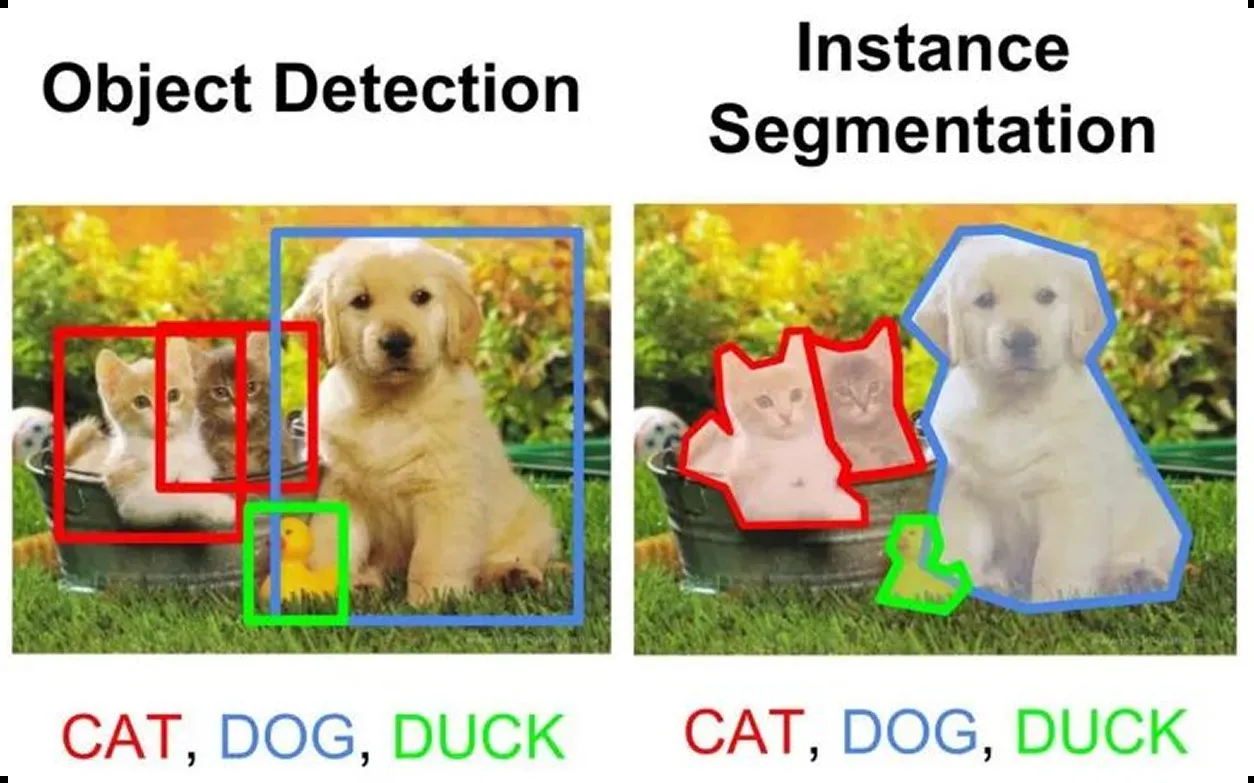
\includegraphics[width=0.95\textwidth]{images/mask_rcnn_fig1.png}
	\captionof{figure}{Mask R-CNN mở rộng bài toán detection sang instance segmentation: mỗi vật thể không chỉ được khoanh bằng bounding box mà còn được tô màu chính xác từng pixel, phân biệt rõ ràng từng cá thể riêng lẻ.}
	\label{fig:mask_rcnn_result}
\end{center}

\textbf{Kiến trúc --- Thêm một nhánh, mở rộng một bài toán.}
Mask R-CNN giữ nguyên toàn bộ pipeline của Faster R-CNN (Backbone → RPN → RoI feature extraction) và chỉ thêm \textit{một nhánh song song} vào detection head. Thay vì hai nhánh (phân loại + hồi quy box), giờ có ba nhánh chạy đồng thời trên mỗi RoI:

\begin{itemize}
	\item \textbf{Classification head}: dự đoán xác suất từng lớp vật thể.
	\item \textbf{Bounding box head}: tinh chỉnh tọa độ hộp bao.
	\item \textbf{Mask head}: dự đoán mask nhị phân pixel-wise cho vật thể.
\end{itemize}

\begin{center}
	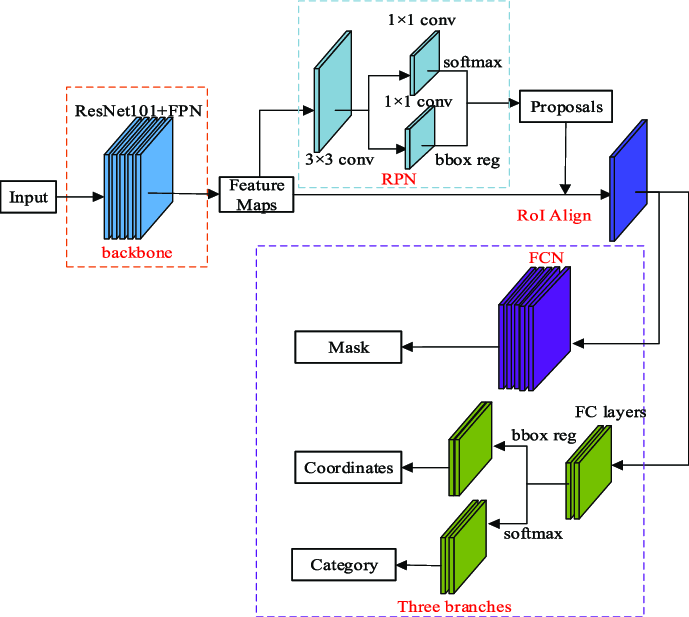
\includegraphics[width=0.95\textwidth]{images/mask_rcnn_diagram.png}
	\captionof{figure}{Kiến trúc Mask R-CNN: backbone + RPN tạo proposals, RoIAlign trích xuất đặc trưng chính xác, ba nhánh song song thực hiện classification, box regression và mask prediction.}
	\label{fig:mask_rcnn}
\end{center}

\textbf{RoIAlign --- Đổi phép làm tròn lấy bilinear interpolation.}
Đây là đóng góp kỹ thuật quan trọng nhất của Mask R-CNN. RoI Pooling trong Fast/Faster R-CNN làm tròn tọa độ khi chiếu vùng đề xuất lên feature map --- sai số lượng tử hóa nhỏ nhưng đủ gây lệch vài pixel khi upscale lên ảnh gốc. Với bounding box, sai lệch vài pixel không ảnh hưởng nhiều. Nhưng với mask pixel-wise, đó là thảm họa.

\textbf{RoIAlign} giải quyết bằng cách \textit{không bao giờ làm tròn}: thay vì snap tọa độ về pixel gần nhất, nó lấy mẫu tại các điểm tọa độ thực (float) và dùng \textbf{bilinear interpolation} để tính giá trị tại đó:
\[
F(x, y) = \sum_{i \in \{0,1\},\, j \in \{0,1\}} w_{ij} \cdot F\!\left(\lfloor x \rfloor + i,\; \lfloor y \rfloor + j\right)
\]
trong đó $w_{ij}$ là trọng số nội suy tỷ lệ với khoảng cách từ $(x,y)$ đến từng điểm lưới lân cận.

\begin{center}
	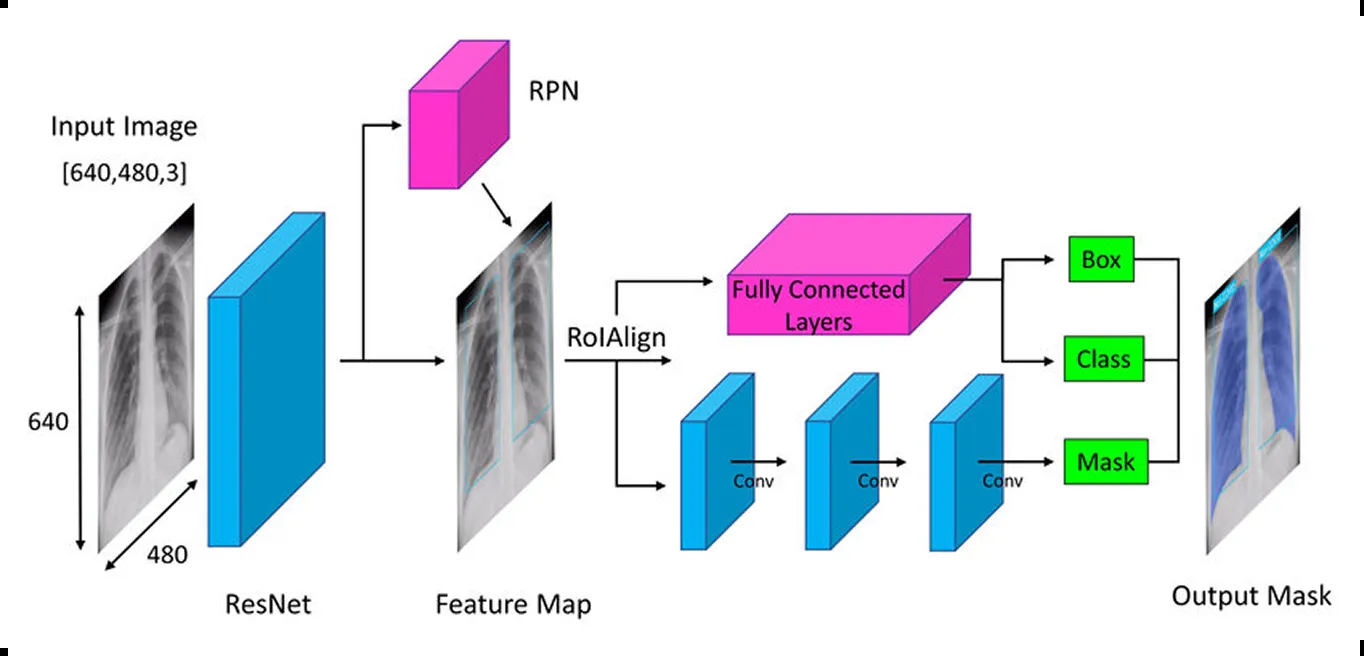
\includegraphics[width=0.90\textwidth]{images/mask_rcnn_fig2.png}
	\captionof{figure}{So sánh RoI Pooling và RoIAlign. RoI Pooling làm tròn tọa độ (đường kẻ đứt) gây lệch vùng; RoIAlign dùng bilinear interpolation tại tọa độ thực, căn chỉnh chính xác feature với vùng trong ảnh gốc.}
	\label{fig:roialign}
\end{center}

Kết quả: mask head nhận được đặc trưng được căn chỉnh hoàn hảo với vùng vật thể --- gradient mượt, không còn sai số tích lũy. Chỉ riêng việc đổi từ RoI Pooling sang RoIAlign đã cải thiện mask AP thêm \textbf{3 điểm}.

\textbf{Mask head --- Dự đoán mask bằng FCN.}
Mask head là một \textbf{Fully Convolutional Network} nhỏ (không có fully-connected layer) nhận đặc trưng $14 \times 14$ từ RoIAlign và xuất ra tensor mask $K \times 28 \times 28$, trong đó $K$ là số lớp vật thể. Mỗi trong $K$ kênh là một binary mask dự đoán độc lập cho lớp đó.

Điểm đặc biệt: Mask R-CNN \textit{không} cho mask và classification cạnh tranh nhau. Mask head dự đoán $K$ mask \textit{đồng thời cho tất cả lớp}, còn classification head quyết định \textit{lớp nào} được chọn. Loss mask chỉ tính trên lớp ground-truth:
\[
L_{\text{mask}} = -\frac{1}{m^2} \sum_{u,v} \left[ M^*_{uv} \log \hat{M}_{uv} + (1 - M^*_{uv}) \log(1 - \hat{M}_{uv}) \right]
\]

Cách tiếp cận này --- gọi là \textbf{decouple mask khỏi classification} --- tránh mask của một lớp bị ảnh hưởng bởi nhãn của lớp khác, giúp mỗi pixel được học như một bài toán binary classification độc lập.

\begin{center}
	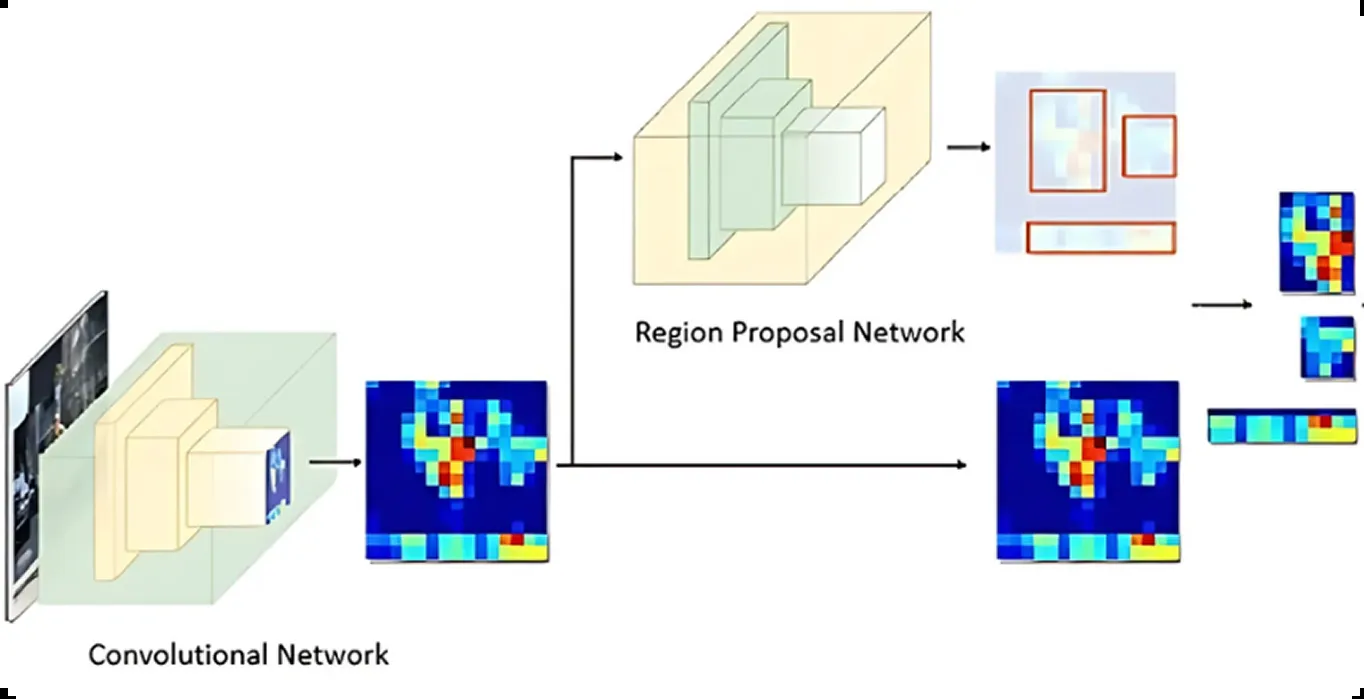
\includegraphics[width=0.85\textwidth]{images/mask_rcnn_fig3.png}
	\captionof{figure}{Mask head trong Mask R-CNN: một FCN nhỏ nhận đặc trưng $14\times14$, xuất mask $K\times28\times28$. Loss chỉ áp dụng trên kênh tương ứng với ground-truth class, không ảnh hưởng qua lại giữa các lớp.}
	\label{fig:mask_head}
\end{center}

\textbf{Hàm mất mát --- Ba nhiệm vụ, một lần tối ưu.}
Toàn bộ mạng được huấn luyện end-to-end với loss tổng hợp:
\[
L = L_{\text{cls}} + L_{\text{box}} + L_{\text{mask}}
\]
Ba thành phần này độc lập và không cạnh tranh nhau: $L_{\text{cls}}$ (cross-entropy) hướng dẫn classification head, $L_{\text{box}}$ (Smooth L1) hướng dẫn box regression, và $L_{\text{mask}}$ (binary cross-entropy per-pixel) hướng dẫn mask head. Mask branch cung cấp tín hiệu gradient dày đặc (dense) từ $28 \times 28 = 784$ pixel mỗi RoI, giúp backbone học biểu diễn không gian phong phú hơn.

\begin{center}
	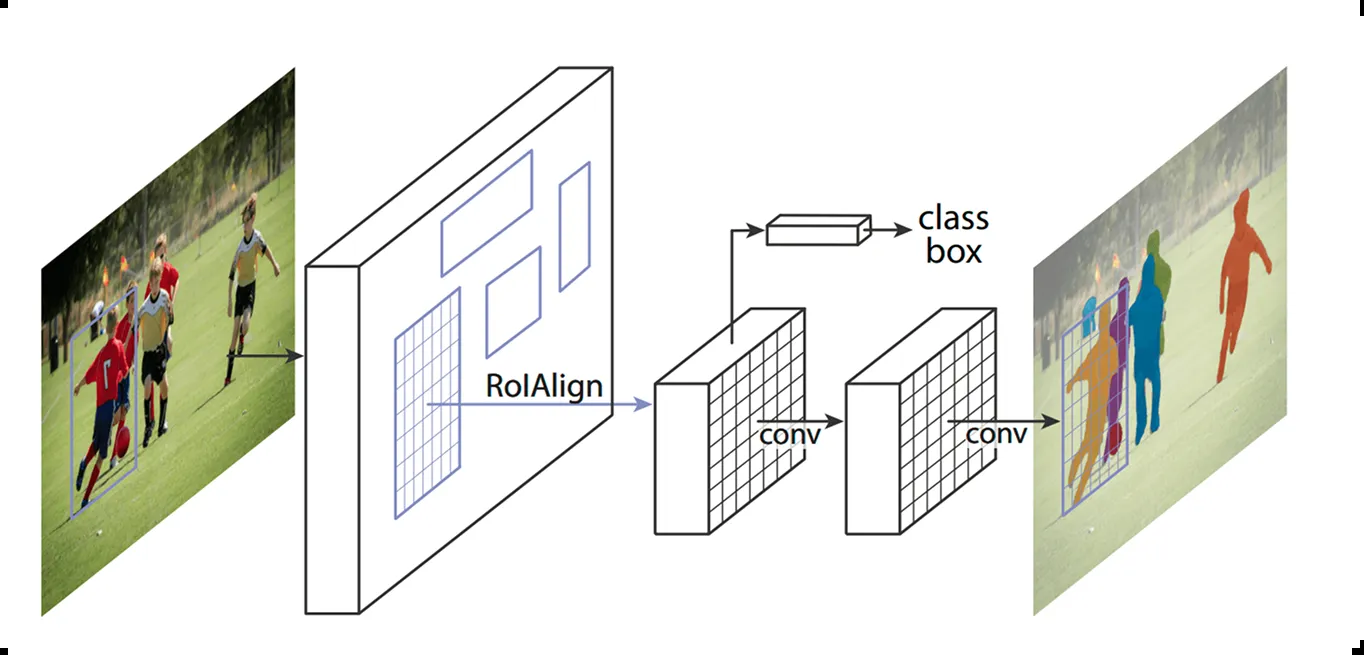
\includegraphics[width=0.90\textwidth]{images/mask_rcnn_fig4.png}
	\captionof{figure}{Ví dụ kết quả Mask R-CNN trên nhiều loại ảnh khác nhau: mỗi instance được tô màu riêng biệt, kể cả khi các vật thể chồng lấp lên nhau.}
	\label{fig:mask_rcnn_results2}
\end{center}

\begin{mdframed}[style=infobox]
\textbf{Kết quả và ứng dụng thực tế}

Mask R-CNN đạt \textbf{37.1\% mask AP} và \textbf{39.8\% box AP} trên COCO test-dev với ResNet-101-FPN backbone, vượt trội mọi phương pháp instance segmentation trước đó. Tốc độ khoảng \textbf{5 FPS} trên GPU --- đủ dùng cho nhiều ứng dụng không yêu cầu real-time.

Mô hình này trở thành nền tảng cho hàng loạt ứng dụng quan trọng:
\begin{itemize}
	\item \textbf{Y tế}: phân đoạn khối u, tế bào, cơ quan trong ảnh MRI/CT với độ chính xác pixel
	\item \textbf{Xe tự lái}: phân biệt từng người đi bộ, xe máy, biển báo riêng lẻ ngay cả khi chồng lấp
	\item \textbf{Bảo tồn động vật}: theo dõi từng cá thể động vật quý hiếm trong môi trường tự nhiên
	\item \textbf{Kiểm soát chất lượng}: phát hiện khuyết tật chính xác đến từng pixel trên dây chuyền sản xuất
\end{itemize}
\end{mdframed}


Họ R-CNN đại diện cho một quá trình tiến hóa mang tính hệ thống trong phát hiện vật thể, trong đó mỗi thế hệ mô hình không chỉ cải thiện hiệu năng mà còn tái định nghĩa cách bài toán được hình thức hóa (formulation) và tối ưu hóa.

Khởi đầu với \textbf{R-CNN (2014)} \cite{Girshick2014}, bài toán phát hiện được phân rã thành ba thành phần rời rạc: sinh vùng đề xuất, trích xuất đặc trưng, và phân loại kết hợp hồi quy. Cách tiếp cận này tận dụng sức mạnh biểu diễn của CNN nhưng vẫn giữ nguyên tư duy pipeline cổ điển. Do đó, mặc dù đạt độ chính xác cao, R-CNN gặp phải hai hạn chế mang tính cấu trúc: (i) chi phí tính toán lớn do lặp lại phép tính CNN trên từng vùng đề xuất, và (ii) không thể tối ưu hóa toàn cục do các thành phần được huấn luyện độc lập.

\textbf{Fast R-CNN (2015)} \cite{Girshick2015} giải quyết nút thắt về tính toán bằng cách tái cấu trúc bài toán: thay vì áp dụng CNN trên từng proposal, toàn bộ ảnh được ánh xạ một lần duy nhất sang không gian đặc trưng, và các vùng quan tâm được trích xuất thông qua phép biến đổi RoI Pooling. Về bản chất, đây là bước chuyển từ \textit{region-wise computation} sang \textit{feature sharing}, giúp giảm độ phức tạp tính toán từ $O(N \cdot \text{CNN})$ xuống $O(\text{CNN} + N)$. Đồng thời, việc tích hợp classification và bounding box regression vào một hàm mất mát thống nhất đã đưa bài toán tiến gần hơn tới huấn luyện end-to-end. Tuy nhiên, sự phụ thuộc vào Selective Search cho thấy pipeline vẫn chưa hoàn toàn khả vi và còn tồn tại một thành phần ngoại lai không thể học được.

Bước ngoặt thực sự đến với \textbf{Faster R-CNN (2016)} \cite{Ren2015}, khi quá trình sinh vùng đề xuất được nội tại hóa thành một bài toán học thông qua Region Proposal Network (RPN). Về mặt bản chất, Faster R-CNN chuyển đổi bài toán từ \textit{proposal generation bằng heuristic} sang \textit{dense prediction trên không gian anchor}, trong đó mỗi anchor đóng vai trò như một giả thuyết (hypothesis) về vị trí và kích thước vật thể. Điều này cho phép mô hình học đồng thời hai nhiệm vụ: phân loại objectness và hồi quy vị trí, dưới một khung tối ưu hóa thống nhất. Quan trọng hơn, việc chia sẻ feature giữa RPN và detector chính không chỉ giảm chi phí tính toán mà còn tạo ra một dạng \textit{multi-task learning}, trong đó các tín hiệu gradient từ cả proposal và detection cùng định hình representation của backbone.

Nhìn tổng thể, sự tiến hóa từ R-CNN → Fast R-CNN → Faster R-CNN phản ánh một xu hướng rõ ràng: chuyển từ pipeline rời rạc sang mô hình học thống nhất, từ heuristic sang học có giám sát, và từ tính toán lặp lại sang chia sẻ đặc trưng. Các cải tiến như RoI Pooling và RPN không chỉ là tối ưu kỹ thuật, mà còn là những bước tiến trong cách biểu diễn và giải bài toán phát hiện vật thể.

Bài học quan trọng rút ra là: hiệu năng cao trong phát hiện vật thể không chỉ đến từ kiến trúc mạng mạnh hơn, mà còn từ việc thiết kế lại bài toán sao cho toàn bộ pipeline trở nên khả vi, có thể tối ưu hóa end-to-end, và tận dụng được sự chia sẻ thông tin giữa các tác vụ liên quan. Chính những nguyên lý này đã đặt nền tảng cho các bộ phát hiện một giai đoạn hiện đại như YOLO, SSD và RetinaNet, nơi toàn bộ quá trình phát hiện được mô hình hóa như một bài toán hồi quy và phân loại duy nhất trên không gian đặc trưng.

\begin{center}
	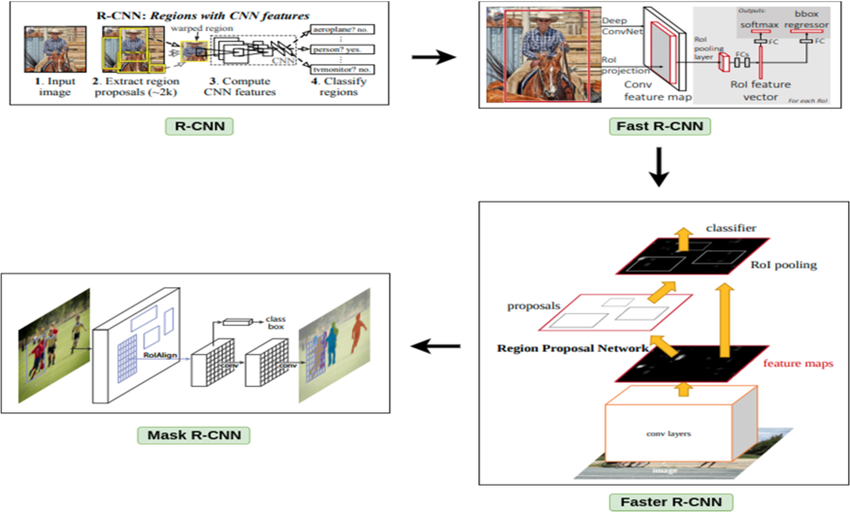
\includegraphics[width=0.95\textwidth]{images/rcnn_evolution_diagram.png}
	\captionof{figure}{Tổng quan quá trình phát triển của họ R-CNN: từ R-CNN → Fast R-CNN → Faster R-CNN. Mỗi bước cải tiến tập trung vào tăng tốc độ, đơn giản hóa pipeline, và hướng tới huấn luyện end-to-end.}
	\label{fig:rcnn_evolution}
\end{center}

\subsubsection{Các bộ phát hiện Một giai đoạn: Nhanh và Hiệu quả}
\label{subsubsec:one_stage_detectors}

\paragraph{YOLO (You Only Look Once, 2016–nay):}
Họ mô hình \textbf{YOLO} \cite{Redmon2016} của Joseph Redmon đã khởi xướng một triết lý hoàn toàn khác: coi phát hiện vật thể như một bài toán hồi quy duy nhất, end-to-end và single-shot.

\textbf{Nguyên lý cốt lõi:} Ảnh đầu vào được chia thành một lưới $S \times S$. Mỗi ô lưới dự đoán $B$ bounding box, confidence score, và xác suất các lớp của vật thể có tâm nằm trong ô đó. Tất cả dự đoán được thực hiện trong \textbf{một lần forward pass}, từ đó đạt tốc độ thời gian thực cao.

\begin{itemize}
	\item \textit{Loss function cơ bản (YOLOv1):}
	\begin{equation}
		\begin{split}
			\mathcal{L} &= \lambda_{\text{coord}} \sum_{i=0}^{S^2} \sum_{j=0}^{B} \mathbf{1}_{ij}^{\text{obj}} 
			\Big[ (x_i - \hat{x}_i)^2 + (y_i - \hat{y}_i)^2 \Big] \\
			&+ \lambda_{\text{coord}} \sum_{i=0}^{S^2} \sum_{j=0}^{B} \mathbf{1}_{ij}^{\text{obj}} 
			\Big[ (\sqrt{w_i} - \sqrt{\hat{w}_i})^2 + (\sqrt{h_i} - \sqrt{\hat{h}_i})^2 \Big] \\
			&+ \sum_{i=0}^{S^2} \sum_{j=0}^{B} \mathbf{1}_{ij}^{\text{obj}} (C_i - \hat{C}_i)^2 \\
			&+ \lambda_{\text{noobj}} \sum_{i=0}^{S^2} \sum_{j=0}^{B} \mathbf{1}_{ij}^{\text{noobj}} (C_i - \hat{C}_i)^2 \\
			&+ \sum_{i=0}^{S^2} \mathbf{1}_{i}^{\text{obj}} \sum_{c \in \text{classes}} (p_i(c) - \hat{p}_i(c))^2
		\end{split}
	\end{equation}
	
	\item \textit{Tiến hóa các phiên bản YOLO:}
	\begin{itemize}
		\item \textbf{YOLOv1 (2016):} 
		\begin{itemize}
			\item Backbone: Darknet-19, đơn giản, 19 conv + 5 max-pooling.
			\item Dự đoán trực tiếp tọa độ và class probabilities.
			\item Hạn chế: vật thể nhỏ khó detect, không dùng anchor boxes.
		\end{itemize}
		
		\item \textbf{YOLOv2 / YOLOv3 (2017–2018):} 
		\begin{itemize}
			\item Giới thiệu \textbf{anchor boxes}: dự đoán offsets, cải thiện dự đoán vật thể nhỏ và đa tỉ lệ.
			\item Multi-scale prediction: dự đoán từ nhiều feature map khác nhau.
			\item Backbone: Darknet-19 (v2), Darknet-53 (v3) với residual connections.
			\item Loss function nâng cao: GIoU hoặc CIoU thay cho MSE bounding box.
		\end{itemize}
		
		\item \textbf{YOLOv4 / YOLOv5 (2020–2021):} 
		\begin{itemize}
			\item Backbone CSPNet (Cross Stage Partial) tăng hiệu năng tính toán.
			\item Neck: PANet (Path Aggregation Network) cho multi-scale feature fusion.
			\item Augmentation mạnh: mosaic, mixup, hue-saturation-jitter, random scaling.
			\item Optimizer: AdamW, learning rate scheduler, label smoothing.
			\item Giữ balance speed–accuracy, tối ưu cho GPU.
		\end{itemize}
		
		\item \textbf{YOLOv6–v8 (2022–2024):} 
		\begin{itemize}
			\item Anchor-free hoặc dynamic anchor trong một số phiên bản.
			\item Loss function nâng cao: Varifocal Loss, CIoU/Focal Loss, cải thiện learning khi class imbalance.
			\item Edge optimization: inference nhanh (>100 FPS), tensor cores, INT8/FP16.
			\item Backbone \& Neck: Efficient CSP, attention blocks (CBAM, SPP), multi-scale prediction.
			\item End-to-end pipeline hoàn thiện, dễ triển khai trên nhiều nền tảng.
		\end{itemize}
	\end{itemize}
	
	\item \textit{Bài học rút ra:}  
	YOLO đã biến phát hiện vật thể từ bài toán nhiều giai đoạn (R-CNN) thành single-shot, end-to-end, và tiếp tục phát triển để xử lý đa dạng tỉ lệ, vật thể nhỏ, class imbalance, đồng thời tối ưu hóa cho tốc độ và hiệu năng. Đây là lý do nó trở thành chuẩn mực trong các ứng dụng thời gian thực từ YOLOv1 → YOLOv8.
	
	
\end{itemize}

\paragraph{YOLO (You Only Look Once, 2016–nay):}

Họ mô hình \textbf{YOLO} \cite{Redmon2016} do Joseph Redmon đề xuất đã định hình lại bài toán phát hiện vật thể bằng cách chuyển từ pipeline nhiều giai đoạn sang một mô hình \textbf{single-shot, end-to-end}. Thay vì sinh proposal rồi phân loại như R-CNN, YOLO coi phát hiện vật thể là một bài toán hồi quy trực tiếp từ ảnh đầu vào sang các bounding box và xác suất lớp.

---

\textbf{Nguyên lý cốt lõi:}

Ảnh đầu vào được chia thành lưới $S \times S$. Mỗi ô lưới chịu trách nhiệm dự đoán các vật thể có tâm nằm trong nó. Với mỗi ô, mô hình dự đoán:
\begin{itemize}
\item $B$ bounding boxes $(x, y, w, h)$
\item Objectness score $P(object)$
\item Xác suất lớp $P(class \mid object)$
\end{itemize}

Điểm confidence cuối cùng:
\[
score = P(object) \cdot P(class)
\]

Toàn bộ dự đoán được thực hiện trong \textbf{một lần forward pass}, giúp YOLO đạt tốc độ thời gian thực.

---

\textbf{Pipeline tổng thể của YOLO:}

\textit{Forward pass:}
\begin{enumerate}
\item Input image $\rightarrow$ resize (e.g. $640 \times 640$)
\item Backbone $\rightarrow$ trích xuất feature map:
\[
F \in \mathbb{R}^{C \times H \times W}
\]
\item Neck (FPN/PAN):
\begin{itemize}
	\item Kết hợp đặc trưng đa tỉ lệ
	\item Sinh ra các feature maps: $P_3, P_4, P_5$
\end{itemize}
\item Detection Head:
\begin{itemize}
	\item Với mỗi grid cell: dự đoán $(x, y, w, h)$, objectness và class probabilities
\end{itemize}
\end{enumerate}

\textit{Post-processing:}
\begin{itemize}
\item Decode bounding box từ offset
\item Tính confidence score
\item Áp dụng \textbf{Non-Maximum Suppression (NMS)} để loại bỏ box trùng lặp
\end{itemize}

---

\textbf{Kiến trúc tổng thể: Backbone – Neck – Head}

\textit{Backbone:}
\begin{itemize}
\item Ví dụ: Darknet-19, Darknet-53, CSPNet
\item Bao gồm các convolutional layers với BatchNorm và activation
\item Sử dụng residual connections:
\[
y = F(x) + x
\]
\item Vai trò: trích xuất đặc trưng ngữ nghĩa từ ảnh
\end{itemize}

\textit{Neck:}
\begin{itemize}
\item Feature Pyramid Network (FPN): kết hợp thông tin từ các tầng sâu và nông
\item Path Aggregation Network (PAN): bổ sung bottom-up path
\item Vai trò: cải thiện khả năng phát hiện vật thể đa tỉ lệ, đặc biệt là vật thể nhỏ
\end{itemize}

\textit{Detection Head:}

Output tensor có dạng:
\[
S \times S \times (B \cdot (5 + C))
\]

Trong đó:
\begin{itemize}
\item $4$: tọa độ bounding box
\item $1$: objectness
\item $C$: số lớp
\end{itemize}

---

\textbf{Anchor-based vs Anchor-free:}

\textit{Anchor-based (YOLOv2–v5):}

Bounding box được dự đoán dưới dạng offset:
\[
\begin{aligned}
b_x &= \sigma(t_x) + c_x \\
b_y &= \sigma(t_y) + c_y \\
b_w &= p_w e^{t_w} \\
b_h &= p_h e^{t_h}
\end{aligned}
\]

Trong đó:
\begin{itemize}
\item $(c_x, c_y)$: vị trí ô lưới
\item $(p_w, p_h)$: anchor box
\item $(t_x, t_y, t_w, t_h)$: output của mạng
\end{itemize}

Anchor giúp mô hình học offset nhỏ, tăng tốc hội tụ và encode prior về kích thước vật thể.

\textit{Anchor-free (YOLOv8):}

\begin{itemize}
\item Không sử dụng anchor boxes
\item Dự đoán trực tiếp center point và khoảng cách tới 4 cạnh (l, t, r, b)
\end{itemize}

Ưu điểm:
\begin{itemize}
\item Đơn giản hóa thiết kế
\item Không cần tuning anchor
\item Khả năng tổng quát hóa tốt hơn
\end{itemize}

---

\textbf{Hàm loss: từ MSE đến IoU-based}

\textit{YOLOv1:} sử dụng MSE cho cả localization và classification.

\textit{YOLO hiện đại:}

\begin{itemize}
\item \textbf{Localization loss:} IoU-based (GIoU, DIoU, CIoU)
\end{itemize}

Ví dụ CIoU:
\[
\mathcal{L}_{CIoU} = 1 - IoU + \frac{\rho^2(b, b^{gt})}{c^2} + \alpha v
\]

\begin{itemize}
\item \textbf{Classification loss:} Binary Cross-Entropy hoặc Focal Loss
\end{itemize}

Focal Loss:
\[
FL(p) = -\alpha (1 - p)^\gamma \log(p)
\]

Giúp xử lý bài toán mất cân bằng lớp.

---

\textbf{Label assignment:}

\textit{Static assignment (YOLOv3–v5):}
\begin{itemize}
\item Mỗi ground truth được gán cho anchor có IoU cao nhất
\end{itemize}

\textit{Dynamic assignment (YOLOv7–v8):}
\begin{itemize}
\item Sử dụng các phương pháp như SimOTA
\item Một ground truth có thể gán cho nhiều prediction
\end{itemize}

Giúp tăng số lượng positive samples và cải thiện độ ổn định khi huấn luyện.

---

\textbf{Non-Maximum Suppression (NMS):}

\begin{itemize}
\item Loại bỏ các bounding box trùng lặp dựa trên IoU
\end{itemize}

Các biến thể:
\begin{itemize}
\item Soft-NMS
\item DIoU-NMS
\end{itemize}

---

\textbf{Tiến hóa các phiên bản YOLO:}

\begin{itemize}
	\item \textbf{YOLOv1 (2016 -- Redmon et al.):}
	\begin{itemize}
		\item \textbf{Kiến trúc:} Single-stage, end-to-end detector; chia ảnh thành lưới $S \times S$ (thường $7 \times 7$), mỗi cell dự đoán trực tiếp 2 bounding boxes, confidence score và class probabilities (không sử dụng anchor boxes, không có neck tách biệt rõ ràng). Backbone gồm 24 convolutional layers và 2 fully connected layers, lấy cảm hứng từ GoogLeNet.
		
		\item \textbf{Thuật toán:} Hàm loss sử dụng squared-error cho cả localization, confidence và classification, tối ưu đồng thời trong một bước huấn luyện.
		
		\item \textbf{Quy trình và cải tiến:} Inference chỉ cần một forward pass, đạt tốc độ thời gian thực (khoảng 45 FPS trên VOC). Việc sử dụng toàn bộ ngữ cảnh ảnh giúp giảm false positives. \textbf{Hạn chế:} hiệu suất kém đối với vật thể nhỏ, khó xử lý nhiều đối tượng trong cùng một cell, và độ chính xác localization còn hạn chế (mAP@0.5 $\approx 63.4\%$ trên VOC).
	\end{itemize}
	
	\item \textbf{YOLOv2--v3 (2017--2018 -- Redmon et al.):}
	\begin{itemize}
		\item \textbf{Kiến trúc:} Giới thiệu anchor boxes (được khởi tạo bằng k-means clustering trên dataset) và dự đoán offsets thay vì tọa độ tuyệt đối. Áp dụng multi-scale prediction; cụ thể YOLOv3 dự đoán trên 3 tỉ lệ thông qua upsampling và concatenation tương tự FPN. Backbone được nâng cấp từ Darknet-19 (v2) lên Darknet-53 (v3) với residual connections. Bắt đầu xuất hiện cơ chế feature fusion đa tỉ lệ.
		
		\item \textbf{Thuật toán:} Sử dụng Batch Normalization và high-resolution classifier với đầu vào $448 \times 448$. YOLOv3 thay softmax bằng logistic classifier độc lập cho từng lớp (multi-label). Áp dụng multi-scale training trong khoảng $320$ đến $608$ pixels.
		
		\item \textbf{Quy trình và cải tiến:} Huấn luyện ổn định hơn và cải thiện khả năng phát hiện vật thể nhỏ. Inference vẫn đạt tốc độ thời gian thực (khoảng 30--67 FPS). Hiệu năng đạt mAP@0.5 $\approx 76.8\%$ (VOC, YOLOv2) và mAP@0.5 $\approx 57.9\%$ (COCO, YOLOv3). Đồng thời hỗ trợ huấn luyện kết hợp detection và classification (YOLO9000).
	\end{itemize}
	
	\item \textbf{YOLOv4--v5 (2020--2021 -- Bochkovskiy et al. \& Ultralytics):}
	\begin{itemize}
		\item \textbf{Kiến trúc:} Chuẩn hóa thành ba thành phần: backbone--neck--head. Backbone sử dụng CSPDarknet-53 (YOLOv4) hoặc CSP-based architecture với SPPF (YOLOv5, tối ưu hơn SPP). Neck kết hợp SPP và PANet (Path Aggregation Network) để tăng cường feature fusion đa tỉ lệ. Detection head vẫn theo hướng anchor-based tương tự YOLOv3.
		
		\item \textbf{Thuật toán:} Áp dụng Bag of Freebies (Mosaic, MixUp, CutMix, Label Smoothing, DropBlock) và Bag of Specials (Mish activation, CIoU loss, Self-Adversarial Training). YOLOv5 bổ sung auto-anchor, tối ưu siêu tham số (hyperparameter evolution) và được triển khai bằng PyTorch.
		
		\item \textbf{Quy trình và cải tiến:} Các kỹ thuật augmentation như Mosaic giúp tăng đáng kể độ đa dạng dữ liệu huấn luyện. Inference nhanh và dễ triển khai (hỗ trợ ONNX, TensorRT). SPPF giúp giảm chi phí tính toán và bộ nhớ. Hiệu năng đạt khoảng mAP@0.5:0.95 $\approx 43.5\%$ (YOLOv4) và $\approx 50\%$ (YOLOv5) trên COCO. Cải thiện đáng kể bài toán vật thể nhỏ và độ ổn định huấn luyện.
	\end{itemize}
	
	\item \textbf{YOLOv6--v8 (2022--2023 -- Meituan, WongKinYiu \& Ultralytics):}
	\begin{itemize}
		\item \textbf{Kiến trúc:} Xu hướng chuyển sang anchor-free hoặc hybrid. Backbone lần lượt sử dụng EfficientRep (YOLOv6, dựa trên RepVGG re-parameterization), E-ELAN (YOLOv7) và C2f module (YOLOv8). Neck sử dụng Rep-PAN hoặc FPN-style. Detection head dạng decoupled (tách riêng classification và regression) và anchor-free trong YOLOv8.
		
		\item \textbf{Thuật toán:} Sử dụng các hàm loss nâng cao như Varifocal Loss, GIoU/SIoU và Distribution Focal Loss (DFL). Label assignment được cải tiến với Task-Aligned Learning (TAL) và các chiến lược dynamic assignment. YOLOv8 hỗ trợ đa nhiệm (detection, segmentation, pose estimation, classification, oriented bounding box).
		
		\item \textbf{Quy trình và cải tiến:} Huấn luyện với dynamic label assignment, exponential moving average (EMA) và self-distillation. Inference được tối ưu nhờ re-parameterization (gộp các lớp convolution khi deploy) và quantization (FP16, INT8). Hiệu năng đạt mAP@0.5:0.95 trên COCO vượt $53\%$ với tốc độ 60--80 FPS. Cải thiện đáng kể gradient flow và khả năng phát hiện vật thể nhỏ.
	\end{itemize}
	
	\item \textbf{YOLOv9--v11 (2024--2025 -- Wang et al. \& Ultralytics):}
	\begin{itemize}
		\item \textbf{Kiến trúc:} Tối ưu hóa gradient flow và hiệu quả biểu diễn. YOLOv9 giới thiệu GELAN (Generalized ELAN) và PGI (Programmable Gradient Information) nhằm giảm hiện tượng information bottleneck. YOLOv10 sử dụng spatial-channel decoupled downsampling và lightweight head. YOLOv11 bổ sung các module như C3k2 và C2PSA để cải thiện khả năng chú ý không gian.
		
		\item \textbf{Thuật toán:} YOLOv10 hỗ trợ NMS-free end-to-end inference thông qua cơ chế dual label assignment (one-to-many trong huấn luyện và one-to-one trong suy luận). Các phiên bản mới tiếp tục sử dụng các biến thể focal loss và distribution-based loss để tối ưu hóa quá trình học.
		
		\item \textbf{Quy trình và cải tiến:} Cải thiện khả năng lan truyền gradient (PGI) giúp hội tụ nhanh và ổn định hơn. YOLOv10 giảm độ trễ suy luận đáng kể nhờ loại bỏ bước NMS. YOLOv11 đạt hiệu năng cao với số lượng tham số giảm, cân bằng tốt giữa tốc độ và độ chính xác. Hiệu năng trên COCO vượt mAP@0.5:0.95 $54\%$, phù hợp cho các ứng dụng thời gian thực và triển khai trên edge devices.
	\end{itemize}
	```
	
\end{itemize}


---

\textbf{Insight quan trọng:}

Thành công của YOLO không chỉ đến từ việc là mô hình single-shot, mà là sự kết hợp của:
\begin{itemize}
\item Dense prediction trên toàn ảnh
\item Multi-scale feature fusion (FPN/PAN)
\item IoU-based regression loss
\item Anchor-based hoặc anchor-free design
\item Backbone tối ưu hóa cho hiệu năng tính toán
\end{itemize}

Nhờ đó, YOLO đạt được sự cân bằng tối ưu giữa tốc độ và độ chính xác, trở thành chuẩn mực cho các ứng dụng phát hiện vật thể thời gian thực.


\paragraph{SSD (Single Shot MultiBox Detector, 2016):}

\textbf{SSD} \cite{Liu2016} là một trong những mô hình phát hiện vật thể một giai đoạn (single-stage) quan trọng, đóng vai trò cầu nối giữa YOLOv1 và các detector hiện đại. SSD kết hợp triết lý \textit{single-shot detection} với \textit{multi-scale feature representation}, cho phép đạt được sự cân bằng hiệu quả giữa tốc độ suy luận và độ chính xác.

---

\textbf{Nguyên lý cốt lõi:}

Khác với YOLOv1 chỉ sử dụng một feature map duy nhất, SSD thực hiện dự đoán trên nhiều feature maps ở các mức độ trừu tượng khác nhau trong mạng CNN. Cụ thể:

\begin{itemize}
	\item Các feature map có độ phân giải cao (shallow layers) được sử dụng để phát hiện vật thể nhỏ.
	\item Các feature map có độ phân giải thấp (deep layers) được sử dụng để phát hiện vật thể lớn.
	\item Tại mỗi vị trí trên mỗi feature map, mô hình dự đoán một tập các bounding boxes cố định gọi là \textbf{default boxes} (hay anchor boxes), với nhiều tỉ lệ và aspect ratios khác nhau.
\end{itemize}

Giả sử có $m$ feature maps với kích thước khác nhau, tổng số bounding boxes được dự đoán là:

\begin{equation}
	N_{boxes} = \sum_{k=1}^{m} H_k \cdot W_k \cdot A_k
\end{equation}

trong đó $H_k, W_k$ là chiều cao và chiều rộng của feature map thứ $k$, và $A_k$ là số default boxes tại mỗi vị trí.

---

\textbf{Kiến trúc tổng thể:}

SSD bao gồm ba thành phần chính: \textit{backbone, extra feature layers và prediction heads}.

\textit{Backbone:}
\begin{itemize}
	\item Thường sử dụng VGG-16 (được cắt bỏ fully connected layers)
	\item Các layer như conv4\_3 và conv7 được sử dụng trực tiếp để dự đoán
\end{itemize}

\textit{Extra feature layers:}
\begin{itemize}
	\item Các convolutional layers bổ sung được thêm vào sau backbone
	\item Mỗi layer có kích thước nhỏ dần (ví dụ: $38 \times 38$, $19 \times 19$, $10 \times 10$, ...)
	\item Cho phép mô hình học biểu diễn đa tỉ lệ
\end{itemize}

\textit{Prediction heads:}
\begin{itemize}
	\item Mỗi feature map được gắn với hai convolution:
	\begin{itemize}
		\item Localization head: dự đoán offsets $(\Delta x, \Delta y, \Delta w, \Delta h)$
		\item Confidence head: dự đoán class scores
	\end{itemize}
\end{itemize}

---

\textbf{Thiết kế default boxes (anchor boxes):}

SSD sử dụng một tập các default boxes với nhiều tỉ lệ khác nhau:

\begin{equation}
	s_k = s_{min} + \frac{s_{max} - s_{min}}{m - 1} (k - 1)
\end{equation}

trong đó:
\begin{itemize}
	\item $s_k$: scale của feature map thứ $k$
	\item $s_{min}, s_{max}$: scale tối thiểu và tối đa
\end{itemize}

Aspect ratios thường được chọn:
\[
{1, 2, 3, \tfrac{1}{2}, \tfrac{1}{3}}
\]

Điều này giúp bao phủ tốt các hình dạng vật thể khác nhau.

---

\textbf{Bounding box parameterization:}

SSD không dự đoán trực tiếp tọa độ tuyệt đối, mà dự đoán offsets so với default box:

\begin{align}
	t_x &= \frac{x - d_x}{d_w}, \quad
	t_y = \frac{y - d_y}{d_h} \\
	t_w &= \log \left( \frac{w}{d_w} \right), \quad
	t_h = \log \left( \frac{h}{d_h} \right)
\end{align}

Trong đó:
\begin{itemize}
	\item $(d_x, d_y, d_w, d_h)$: default box
	\item $(x, y, w, h)$: ground truth box
\end{itemize}

---

\textbf{Matching strategy (label assignment):}

SSD sử dụng cơ chế matching giữa default boxes và ground truth dựa trên IoU:

\begin{itemize}
	\item Mỗi ground truth được gán với default box có IoU cao nhất
	\item Các default boxes có IoU $> 0.5$ cũng được gán là positive
\end{itemize}

Kết quả:
\begin{itemize}
	\item Positive samples: dùng cho cả localization và classification
	\item Negative samples: chỉ dùng cho classification
\end{itemize}

---

\textbf{Hard Negative Mining:}

Do số lượng negative samples rất lớn, SSD áp dụng chiến lược:

\begin{itemize}
	\item Sắp xếp negative samples theo confidence loss giảm dần
	\item Chọn tối đa tỷ lệ:
	\[
	\frac{N_{neg}}{N_{pos}} \leq 3
	\]
\end{itemize}

Điều này giúp giảm mất cân bằng lớp và ổn định quá trình huấn luyện.

---

\textbf{Hàm loss tổng thể:}

\begin{equation}
	\mathcal{L}(x, c, l, g) = \frac{1}{N} \left( \mathcal{L}_{conf}(x, c) + \alpha \mathcal{L}_{loc}(x, l, g) \right)
\end{equation}

\textit{Localization loss (Smooth L1):}
\begin{equation}
	\mathcal{L}_{loc} = \sum_{i \in Pos} \sum_{m \in {x,y,w,h}}
	\text{smooth}_{L1}(l_i^m - \hat{g}_i^m)
\end{equation}

\textit{Confidence loss (Softmax cross-entropy):}
\begin{equation}
	\mathcal{L}_{conf} = \sum_{i \in Pos} \underbrace{-\log(\hat{c}_i^{p})}_{\text{positive loss}}
	+ \sum_{i \in Neg} \underbrace{-\log(\hat{c}_i^{0})}_{\text{negative loss}}
\end{equation}

---

\textbf{Pipeline huấn luyện và suy luận:}

\textit{Training:}
\begin{enumerate}
	\item Input image $\rightarrow$ data augmentation (random crop, flip, photometric distortion)
	\item Forward pass qua backbone và extra layers
	\item Matching default boxes với ground truth
	\item Tính loss (loc + conf)
	\item Hard negative mining
	\item Backpropagation
\end{enumerate}

\textit{Inference:}
\begin{enumerate}
	\item Forward pass
	\item Decode bounding boxes từ offsets
	\item Tính confidence scores
	\item Áp dụng Non-Maximum Suppression (NMS)
\end{enumerate}

---

\textbf{Ưu điểm:}

\begin{itemize}
	\item Tốc độ cao (real-time, $\sim 59$ FPS với SSD300)
	\item Kiến trúc đơn giản, dễ triển khai
	\item Multi-scale detection hiệu quả hơn YOLOv1
\end{itemize}

---

\textbf{Hạn chế:}

\begin{itemize}
	\item Hiệu năng với vật thể nhỏ vẫn hạn chế (do thiếu feature fusion mạnh như FPN)
	\item Default boxes cần thiết kế thủ công
	\item Không có cơ chế attention hoặc dynamic assignment
\end{itemize}

---

\textbf{Insight quan trọng:}

SSD cho thấy rằng:
\begin{itemize}
	\item Việc sử dụng \textbf{multi-scale feature maps} là chìa khóa để cải thiện phát hiện vật thể
	\item Anchor-based dense prediction có thể đạt hiệu năng cao mà không cần proposal stage
	\item Hard negative mining là yếu tố quan trọng để xử lý class imbalance
\end{itemize}

Những ý tưởng này đã trở thành nền tảng cho nhiều mô hình hiện đại như RetinaNet (Focal Loss) và các detector dựa trên FPN.

\paragraph{Feature Pyramid Network (FPN, 2017):}
Một trong những thách thức dai dẳng nhất của object detection là \textbf{vật thể đa kích thước}: một con người có thể chiếm 90\% diện tích ảnh hoặc chỉ vài pixel. CNN truyền thống xử lý ảnh theo một tỷ lệ duy nhất --- feature map ở layer sâu giàu ngữ nghĩa nhưng mất độ phân giải không gian, còn feature map ở layer nông có độ phân giải cao nhưng ngữ nghĩa nghèo. \textbf{Feature Pyramid Network (FPN)} \cite{Lin2017FPN} của Lin và cộng sự giải quyết mâu thuẫn này bằng cách xây dựng một \textit{kim tự tháp đặc trưng} kết hợp ưu điểm của cả hai.

\textbf{Hai luồng xử lý bổ sung nhau.}
FPN hoạt động với hai luồng đồng thời trên backbone CNN (thường là ResNet):

\begin{itemize}
    \item \textbf{Bottom-up pathway} (xuôi chiều): Luồng forward pass thông thường của CNN. Khi đi sâu hơn, feature map giảm kích thước (stride tăng) nhưng mỗi pixel mã hóa ngữ nghĩa phong phú hơn. Các tầng output ký hiệu là $\{C_2, C_3, C_4, C_5\}$ với stride $\{4, 8, 16, 32\}$.
    \item \textbf{Top-down pathway} (ngược chiều): Bắt đầu từ $C_5$ (layer sâu nhất, ngữ nghĩa cao nhất), upsample dần lên các độ phân giải lớn hơn. Tại mỗi tầng, feature map được upsample 2× rồi \textit{cộng} với feature map tương ứng từ bottom-up qua một \textbf{lateral connection} ($1 \times 1$ conv để chuẩn hóa số kênh về 256):
\end{itemize}

\[
P_k = \text{Conv}_{1\times1}(C_k) + \text{Upsample}(P_{k+1})
\]

Kết quả là kim tự tháp $\{P_2, P_3, P_4, P_5\}$ --- mỗi tầng có 256 kênh, kết hợp độ phân giải cao từ layer nông và ngữ nghĩa phong phú từ layer sâu.

\textbf{Tại sao FPN hiệu quả?} Hãy nghĩ về nó như thế này: layer $C_5$ ``nhìn thấy'' toàn bộ bức ảnh nhưng mỗi pixel của nó đại diện cho vùng $32 \times 32$ pixel gốc --- tốt cho vật thể lớn, tệ cho vật thể nhỏ. Layer $C_2$ ngược lại --- mỗi pixel chỉ đại diện cho $4 \times 4$ pixel gốc. FPN truyền thông tin từ $C_5$ ngược lên, bổ sung ngữ nghĩa cho các layer nông. Kết quả: detector trên $P_2$ vừa có độ phân giải cao (phát hiện vật thể nhỏ) vừa ``biết'' context toàn cục (nhờ thông tin từ $C_5$). Cải thiện so với single-scale: \textbf{+8 AP trên COCO}.

Mỗi tầng $P_k$ chịu trách nhiệm phát hiện vật thể ở kích thước tương ứng: $P_2$ cho vật thể rất nhỏ ($32^2$ pixel), $P_3$ cho nhỏ, $P_4$ cho trung bình, $P_5$ cho lớn. FPN trở thành backbone tiêu chuẩn cho hầu hết detector hiện đại --- từ Faster R-CNN, Mask R-CNN đến RetinaNet, YOLO v3 trở đi.

\paragraph{RetinaNet và Focal Loss (2017):}
Ngay cả với FPN, các one-stage detector vẫn thua two-stage về độ chính xác. Câu hỏi là: \textit{tại sao?} Năm 2017, Lin và cộng sự (Facebook AI) chỉ ra nguyên nhân gốc rễ không phải là kiến trúc mà là \textbf{mất cân bằng lớp cực độ}: một ảnh thông thường có thể tạo ra $\sim$100.000 anchor, nhưng chỉ $\sim$10 anchor là positive (chứa vật thể thực sự). 99.99\% còn lại là nền.

Cross-entropy thông thường xử lý tất cả anchor bình đẳng. Hàng trăm nghìn anchor nền, dù mỗi cái chỉ góp loss nhỏ, cộng lại áp đảo tín hiệu từ những anchor vật thể hiếm hoi. Mô hình học cách phân loại nền rất giỏi --- nhưng detection thật sự thì không.

\textbf{Focal Loss --- Giải pháp qua một hệ số đơn giản.}
\textbf{RetinaNet} \cite{Lin2017RetinaNet} đề xuất \textbf{Focal Loss}: thêm một hệ số điều chỉnh vào cross-entropy để tự động \textit{giảm trọng số} các mẫu dễ (easy negatives) và \textit{tăng trọng số} các mẫu khó:

\begin{equation}
    \text{FL}(p_t) = -\alpha_t\,(1 - p_t)^{\gamma}\,\log(p_t)
\end{equation}

Trong đó $p_t$ là xác suất dự đoán cho đúng nhãn, $\gamma \geq 0$ là tham số điều chỉnh (thực nghiệm cho thấy $\gamma = 2$ tốt nhất), và $\alpha_t$ cân bằng tần suất giữa positive/negative.

Cơ chế hoạt động của $(1-p_t)^\gamma$ rất trực quan:
\begin{itemize}
    \item \textbf{Anchor nền dễ phân loại} ($p_t \approx 0.99$): $(1 - 0.99)^2 = 0.0001$ --- loss giảm xuống còn 0.01\% so với cross-entropy thông thường.
    \item \textbf{Anchor vật thể khó nhận biết} ($p_t \approx 0.3$): $(1 - 0.3)^2 = 0.49$ --- loss chỉ giảm một chút, vẫn nhận được gradient mạnh để học.
\end{itemize}

Kết quả: mô hình tự động tập trung vào những anchor \textit{thật sự cần học}, không lãng phí gradient vào 99\% nền hiển nhiên. Không cần hard negative mining thủ công như SSD.

\textbf{Kiến trúc RetinaNet.}
RetinaNet kết hợp ba thành phần: backbone \textbf{ResNet-50/101} + \textbf{FPN} tạo feature pyramid $\{P_3, \ldots, P_7\}$ với 256 kênh mỗi tầng; hai \textbf{subnet song song} (không chia sẻ tham số) --- mỗi subnet là 4 lớp Conv $3\times3$:
\begin{itemize}
    \item \textit{Classification subnet}: với mỗi trong $A = 9$ anchor tại mỗi vị trí, dự đoán xác suất $K$ lớp --- output $K \times A$ giá trị, dùng Focal Loss.
    \item \textit{Box regression subnet}: dự đoán 4 offset bounding box cho mỗi anchor --- dùng Smooth L1 loss.
\end{itemize}

Cả hai subnet dùng chung kiến trúc nhưng \textit{không chia sẻ tham số} để mỗi nhiệm vụ được tối ưu độc lập.

\begin{mdframed}[style=infobox]
\textbf{Kết quả và tầm quan trọng của RetinaNet}

RetinaNet với ResNet-101-FPN đạt \textbf{40.8 AP} trên COCO --- vượt Faster R-CNN + FPN (36.2 AP) và nhanh hơn $\sim$5 lần. Đây là lần đầu tiên một one-stage detector vượt two-stage về độ chính xác.

Focal Loss trở thành nền tảng cho hàng loạt hàm loss hiện đại: Quality Focal Loss (QFL), Distribution Focal Loss (DFL) trong GFL, VariFocal Loss trong VarifocalNet --- tất cả đều kế thừa ý tưởng \textit{reweight gradient theo độ khó của mẫu}.
\end{mdframed}

\subsection{Đánh giá mô hình: Precision, Recall và mAP}
\label{subsec:map_evaluation}

Trước khi tiếp tục với các kiến trúc hiện đại, cần hiểu rõ thước đo mà tất cả các mô hình trên đều được so sánh: \textbf{mAP (mean Average Precision)}. Đây là metric tiêu chuẩn trong object detection, nhưng cách tính của nó thường bị giải thích sơ sài. Hãy xây dựng từ nền tảng.

\textbf{Precision và Recall --- Hai mặt của một đồng xu.}
Khi một detector dự đoán một bounding box, có hai câu hỏi: (1) Dự đoán đó có đúng không? (2) Mô hình có bỏ sót vật thể nào không?

Một dự đoán được coi là \textbf{True Positive (TP)} nếu: đúng lớp vật thể \textit{và} IoU với ground-truth $\geq$ ngưỡng (thường 0.5). Nếu không khớp ground-truth nào, đó là \textbf{False Positive (FP)}. Ground-truth không được detect là \textbf{False Negative (FN)}.

\[
\text{Precision} = \frac{TP}{TP + FP} \qquad \text{Recall} = \frac{TP}{TP + FN}
\]

Precision cao nghĩa là ít dự đoán sai; Recall cao nghĩa là ít bỏ sót. Hai đại lượng này thường đánh đổi nhau: hạ ngưỡng confidence → detect nhiều hơn → Recall tăng nhưng Precision giảm.

\textbf{Precision-Recall Curve và Average Precision (AP).}
Bằng cách thay đổi ngưỡng confidence từ 1.0 xuống 0.0, ta thu được một tập các cặp (Precision, Recall). Vẽ lên đồ thị tạo thành \textbf{Precision-Recall curve}. \textbf{Average Precision (AP)} là diện tích dưới đường cong này --- một số duy nhất từ 0 đến 1 tóm tắt hiệu năng của mô hình trên \textit{một lớp vật thể}.

Công thức tính AP theo phương pháp \textit{all-point interpolation} (PASCAL VOC 2010+, COCO):
\[
\text{AP} = \int_0^1 P(r)\, dr \approx \sum_{k} \left( r_k - r_{k-1} \right) \cdot P_{\text{interp}}(r_k)
\]
trong đó $P_{\text{interp}}(r) = \max_{\tilde{r} \geq r} P(\tilde{r})$ là precision nội suy tại mỗi mức recall.

\textbf{mAP --- Trung bình AP trên tất cả lớp.}
\[
\text{mAP} = \frac{1}{C} \sum_{c=1}^{C} \text{AP}_c
\]
trong đó $C$ là số lớp vật thể. Mô hình phát hiện tốt đều lớp (cả vật thể phổ biến lẫn hiếm) sẽ có mAP cao.

\begin{mdframed}[style=infobox]
\textbf{PASCAL VOC vs. COCO: Hai tiêu chuẩn khác nhau}

\textbf{PASCAL VOC}: AP tính tại ngưỡng IoU cố định 0.5 → ký hiệu $\text{AP}_{50}$ hay $\text{mAP@0.5}$. Dễ đạt điểm cao vì cho phép box không quá chính xác.

\textbf{COCO}: Nghiêm ngặt hơn nhiều. $\text{AP}$ là trung bình của AP tại 10 ngưỡng IoU từ 0.50 đến 0.95 (bước 0.05) → ký hiệu $\text{mAP@[0.5:0.95]}$. Mô hình phải dự đoán \textit{chính xác vị trí} mới đạt điểm cao. Ngoài ra COCO còn báo cáo riêng:
\begin{itemize}
    \item $\text{AP}_S$, $\text{AP}_M$, $\text{AP}_L$: AP theo kích thước vật thể (small/medium/large)
    \item $\text{AP}_{50}$, $\text{AP}_{75}$: AP tại ngưỡng IoU cụ thể
\end{itemize}

Khi đọc benchmark: 50 AP trên COCO $\approx$ rất tốt; 73 mAP trên PASCAL VOC cũng tốt --- nhưng hai con số này \textit{không so sánh được} với nhau.
\end{mdframed}

\subsection{Kỷ nguyên Transformer: DETR và các Cải tiến}
\label{subsec:transformer_based_detectors}

Năm 2020, Facebook AI Research đề xuất \textbf{DEtection TRansformer (DETR)} \cite{Carion2020}, đánh dấu một bước chuyển quan trọng trong bài toán phát hiện vật thể: chuyển từ \textit{dense prediction với heuristic} sang \textbf{set prediction end-to-end}. DETR loại bỏ hoàn toàn các thành phần thủ công như anchor boxes, Region Proposal Network (RPN) và Non-Maximum Suppression (NMS), thay vào đó sử dụng Transformer để trực tiếp ánh xạ ảnh đầu vào thành một tập các đối tượng.

---

\paragraph{Bài toán set prediction:}

Khác với các detector truyền thống dự đoán hàng nghìn bounding boxes rồi lọc bằng NMS, DETR mô hình hóa bài toán detection như một phép ánh xạ:

\begin{equation}
	f: \mathcal{I} \rightarrow {(y_i, b_i)}_{i=1}^{N}
\end{equation}

trong đó:
\begin{itemize}
	\item $\mathcal{I}$: ảnh đầu vào
	\item $y_i$: nhãn lớp
	\item $b_i$: bounding box
	\item $N$: số lượng dự đoán cố định (ví dụ 100 object queries)
\end{itemize}

Tập dự đoán này là \textbf{không có thứ tự} (permutation-invariant), do đó cần một cơ chế matching tối ưu để so sánh với ground truth.

---

\paragraph{Kiến trúc tổng thể:}

DETR bao gồm ba thành phần chính: backbone CNN, Transformer encoder-decoder và prediction heads.

\textit{Backbone CNN:}
\begin{itemize}
	\item Sử dụng ResNet-50 hoặc ResNet-101 để trích xuất feature map:
	\[
	F \in \mathbb{R}^{C \times H \times W}
	\]
	\item Feature map được giảm chiều (thường qua $1 \times 1$ convolution)
\end{itemize}

---

\textit{Transformer Encoder:}

Feature map được reshape thành chuỗi:
\[
X \in \mathbb{R}^{(H \cdot W) \times C}
\]

Sau đó bổ sung positional encoding và đưa vào encoder:

\begin{itemize}
	\item Self-attention:
	\[
	\text{Attention}(Q, K, V) = \text{softmax}\left(\frac{QK^T}{\sqrt{d}}\right)V
	\]
	\item Mỗi vị trí học được thông tin ngữ cảnh toàn cục
\end{itemize}

---

\textit{Transformer Decoder và Object Queries:}

Decoder nhận vào:
\begin{itemize}
	\item Output từ encoder (memory)
	\item Một tập các vector học được gọi là \textbf{object queries}:
	\[
	Q \in \mathbb{R}^{N \times d}
	\]
\end{itemize}

Mỗi query tương tác với toàn bộ feature thông qua cross-attention:
\begin{itemize}
	\item Query học cách “tập trung” vào một đối tượng cụ thể
	\item Mỗi query tương ứng với một dự đoán object
\end{itemize}

---

\textit{Prediction Heads:}

Output của mỗi query được đưa qua một feed-forward network (FFN):

\begin{itemize}
	\item Classification head: dự đoán xác suất lớp (bao gồm class "no object")
	\item Regression head: dự đoán bounding box chuẩn hóa $(x, y, w, h)$
\end{itemize}

---

\paragraph{Hungarian Bipartite Matching:}

Để huấn luyện mô hình, DETR sử dụng \textbf{Hungarian matching} để tìm ánh xạ tối ưu giữa tập dự đoán và ground truth.

Chi phí matching được định nghĩa:

\begin{equation}
	\mathcal{L}*{match}(i, j) = - \log p_i(y_j) + \lambda \cdot \mathcal{L}*{box}(b_i, b_j)
\end{equation}

Bài toán matching:

\begin{equation}
	\hat{\sigma} = \arg\min_{\sigma} \sum_{i=1}^{N} \mathcal{L}_{match}(i, \sigma(i))
\end{equation}

trong đó $\sigma$ là một hoán vị.

Ý nghĩa:
\begin{itemize}
	\item Mỗi ground truth được gán với đúng một prediction
	\item Loại bỏ hoàn toàn duplicate predictions $\rightarrow$ không cần NMS
\end{itemize}

---

\paragraph{Hàm loss tổng thể:}

Sau khi matching, loss được tính:

\begin{equation}
	\mathcal{L} = \sum_{i=1}^{N} \left( \mathcal{L}*{cls} + \lambda*{1} \mathcal{L}*{L1} + \lambda*{2} \mathcal{L}_{IoU} \right)
\end{equation}

\begin{itemize}
	\item $\mathcal{L}*{cls}$: cross-entropy (bao gồm class "no object")
	\item $\mathcal{L}*{L1}$: khoảng cách giữa bounding boxes
	\item $\mathcal{L}_{IoU}$: GIoU loss
\end{itemize}

---

\paragraph{Tại sao DETR không cần NMS:}

Trong các mô hình truyền thống:
\begin{itemize}
	\item Nhiều prediction trùng nhau $\rightarrow$ cần NMS
\end{itemize}

Trong DETR:
\begin{itemize}
	\item Hungarian matching đảm bảo mỗi object chỉ được dự đoán một lần
	\item Các query học phân công nhiệm vụ (implicit assignment)
\end{itemize}

$\Rightarrow$ mô hình trở thành \textbf{set predictor thuần túy}.

---

\paragraph{Hạn chế của DETR:}

\begin{itemize}
	\item \textbf{Hội tụ chậm:}
	\begin{itemize}
		\item Matching không ổn định ở giai đoạn đầu
		\item Gradient sparse do one-to-one assignment
	\end{itemize}
	\item \textbf{Hiệu năng kém với vật thể nhỏ:}
	\begin{itemize}
		\item Attention toàn cục trên feature map coarse
		\item Thiếu multi-scale feature mạnh như FPN
	\end{itemize}
	```
	
\end{itemize}

---

\paragraph{Các cải tiến quan trọng:}

\textit{Deformable DETR:}
\begin{itemize}
	\item Thay global attention bằng attention trên một số điểm tham chiếu
	\item Giảm độ phức tạp từ $O(N^2)$ xuống gần tuyến tính
	\item Hỗ trợ multi-scale feature
	\item Cải thiện tốc độ hội tụ và small object detection
\end{itemize}

\textit{DN-DETR và DINO:}
\begin{itemize}
	\item Giới thiệu denoising queries
	\item Ổn định quá trình huấn luyện
	\item Tăng tốc hội tụ đáng kể
\end{itemize}

\textit{Conditional / Anchor DETR:}
\begin{itemize}
	\item Kết hợp ý tưởng anchor vào query
	\item Giúp query hội tụ nhanh hơn
\end{itemize}

---

\paragraph{Insight quan trọng:}

DETR mang lại một góc nhìn hoàn toàn mới:

\begin{itemize}
	\item Detection có thể được mô hình hóa như \textbf{set prediction} thay vì dense classification
	\item Việc loại bỏ heuristic (anchor, NMS) giúp pipeline đơn giản và nhất quán
	\item Transformer cho phép học quan hệ toàn cục giữa các object
\end{itemize}

Tuy nhiên, DETR cũng cho thấy rằng:
\begin{itemize}
	\item One-to-one assignment tuy elegant nhưng gây khó khăn cho optimization
	\item Multi-scale và local inductive bias vẫn rất quan trọng
\end{itemize}

Các biến thể sau này kết hợp giữa Transformer và inductive bias của CNN, tạo ra các mô hình mạnh mẽ hơn, cân bằng giữa tính tổng quát và hiệu quả huấn luyện.

\subsection{YOLO Thế hệ Mới và Các Hướng đi Tiên phong}
\label{subsec:new_generation_yolo}

Bên cạnh sự phát triển liên tục của các phiên bản YOLO truyền thống, những năm gần đây chứng kiến sự xuất hiện của các hướng tiếp cận mới nhằm giải quyết các giới hạn cốt lõi của object detection, bao gồm: phụ thuộc vào thiết kế thủ công, giới hạn tập lớp, và chi phí triển khai. Các mô hình YOLO thế hệ mới không chỉ cải tiến kiến trúc mà còn mở rộng bài toán sang các thiết lập tổng quát hơn như \textit{open-vocabulary detection} và \textit{automated model design}.

---

\paragraph{YOLO-NAS (2023): Neural Architecture Search cho Detection}

\textbf{YOLO-NAS} áp dụng \textbf{Neural Architecture Search (NAS)} để tự động tìm kiếm kiến trúc tối ưu thay vì thiết kế thủ công như các phiên bản YOLO trước đó.

\textit{Nguyên lý:}
\begin{itemize}
	\item Xây dựng một không gian kiến trúc (search space) bao gồm:
	\begin{itemize}
		\item Các block convolution (CSP, bottleneck, depthwise conv)
		\item Kích thước kernel, số channel
		\item Cấu trúc backbone và neck
	\end{itemize}
	
	\item Sử dụng chiến lược tìm kiếm (evolutionary search hoặc gradient-based NAS) để tối ưu:
	\[
	\max_{\mathcal{A}} \big( \text{Accuracy}(\mathcal{A}) - \lambda \cdot \text{Latency}(\mathcal{A}) \big)
	\]
	
	\item Quá trình search được thực hiện dưới ràng buộc tài nguyên (FLOPs, latency, memory)
\end{itemize}

\textit{Kiến trúc:}
\begin{itemize}
	\item Backbone và neck được thiết kế tự động
	\item Head vẫn theo hướng decoupled (classification và regression)
	\item Sử dụng quantization-aware training (QAT) để tối ưu triển khai INT8
\end{itemize}

\textit{Ý nghĩa:}
\begin{itemize}
	\item Loại bỏ phụ thuộc vào kinh nghiệm thiết kế thủ công
	\item Tạo ra các mô hình tối ưu riêng cho từng nền tảng (edge, mobile, server)
\end{itemize}

---

\paragraph{YOLO-World (2024): Open-Vocabulary Detection}

\textbf{YOLO-World} mở rộng bài toán detection từ closed-set sang \textbf{open-vocabulary}, cho phép phát hiện các đối tượng chưa xuất hiện trong dữ liệu huấn luyện.

\textit{Nguyên lý cốt lõi:}

Mô hình kết hợp biểu diễn thị giác với embedding ngôn ngữ từ các mô hình foundation như CLIP:

\begin{itemize}
	\item Ảnh đầu vào được encode thành đặc trưng thị giác:
	\[
	f_v = \phi_{\text{vision}}(I)
	\]
	
	\item Văn bản (prompt) được encode thành embedding ngôn ngữ:
	\[
	f_t = \phi_{\text{text}}(T)
	\]
	
	\item Phân loại dựa trên độ tương đồng cosine:
	\[
	\text{score} = \frac{f_v \cdot f_t}{|f_v| \, |f_t|}
	\]
\end{itemize}

---

\textit{Cơ chế tích hợp với YOLO:}

\begin{itemize}
	\item Detection head không còn dự đoán class cố định
	\item Thay vào đó, dự đoán embedding vector cho mỗi bounding box
	\item So khớp embedding này với embedding văn bản
\end{itemize}

\textit{Ưu điểm:}
\begin{itemize}
	\item Có thể phát hiện object chưa từng thấy (zero-shot detection)
	\item Linh hoạt với input dạng ngôn ngữ tự nhiên
\end{itemize}

\textit{Thách thức:}
\begin{itemize}
	\item Alignment giữa vision và language chưa hoàn hảo
	\item Độ chính xác thấp hơn so với closed-set detection trong một số trường hợp
\end{itemize}

---

\paragraph{Các hướng phát triển mới:}

\textit{1. Automated model design:}
\begin{itemize}
	\item NAS, AutoML giúp tối ưu kiến trúc theo phần cứng
	\item Xu hướng chuyển từ \textit{human-designed} sang \textit{data-driven design}
\end{itemize}

\textit{2. Multi-modal learning:}
\begin{itemize}
	\item Kết hợp hình ảnh, ngôn ngữ và ngữ cảnh
	\item Ứng dụng trong robotics, autonomous systems, AR/VR
\end{itemize}

\textit{3. Efficient inference:}
\begin{itemize}
	\item Quantization (INT8, FP16)
	\item Pruning, knowledge distillation
	\item Tối ưu cho edge devices (Jetson, mobile)
\end{itemize}

\textit{4. Generalization beyond closed-set:}
\begin{itemize}
	\item Open-vocabulary detection
	\item Zero-shot và few-shot learning
	\item Unified models cho nhiều tác vụ (detect, segment, caption)
\end{itemize}

---

\paragraph{Insight quan trọng:}

Các thế hệ YOLO mới cho thấy một sự chuyển dịch quan trọng trong object detection:

\begin{itemize}
	\item Từ \textbf{thiết kế thủ công} sang \textbf{tự động hóa kiến trúc} (NAS)
	\item Từ \textbf{closed-set detection} sang \textbf{open-world perception}
	\item Từ \textbf{vision-only} sang \textbf{multi-modal understanding}
\end{itemize}

Điều này phản ánh xu hướng chung của lĩnh vực thị giác máy tính: xây dựng các hệ thống có khả năng \textbf{hiểu môi trường một cách linh hoạt và tổng quát}, thay vì chỉ giải quyết các bài toán hẹp với tập lớp cố định. Các mô hình như YOLO-World là bước tiến đầu tiên hướng tới một \textbf{universal perception system}, có thể tích hợp nhận diện, mô tả và suy luận trong cùng một kiến trúc.

\subsection{Các Kiến trúc Nhận biết Góc quay và Anchor-Free}
\label{subsec:angle_aware_anchor_free}

\begin{description}
	\item[Phát hiện Vật thể có Góc quay (Rotated Object Detection):] 
	Trong nhiều ứng dụng thực tế như ảnh viễn thám, OCR, hay robot gắp hàng, các vật thể thường không nằm thẳng hàng với trục của ảnh. Thay vì dùng bounding box trục-aligned truyền thống $(x, y, w, h)$, các kiến trúc này dự đoán một bounding box có 5 tham số $(x, y, w, h, \theta)$:
	\begin{itemize}
		\item $\theta$: góc quay của vật thể so với trục x.
		\item Giúp bao quanh đối tượng một cách chặt chẽ hơn, cải thiện IoU và độ chính xác cho vật thể nghiêng hoặc dài.
		\item Các mô hình rotated detection thường cần:
		\begin{itemize}
			\item \textbf{Representation strategies:} sử dụng $R$-box (rotated box) hoặc polygon-based để mô tả hình dạng vật thể.
			\item \textbf{Angle regression loss:} Smooth L1 hoặc IoU-based loss mở rộng cho góc quay, đôi khi kết hợp với Modulo 180/360 để tránh discontinuity.
			\item \textbf{Anchor design (nếu anchor-based):} anchors cần thêm orientation parameter để bao phủ các góc quay phổ biến.
		\end{itemize}
		\item Thường kết hợp với anchor-based hoặc anchor-free approaches, tùy kiến trúc.
	\end{itemize}
	
	\item[Anchor-based vs. Anchor-free:] 
	Cuộc tranh luận về việc có nên sử dụng "khung neo" hay không vẫn tiếp diễn.
	\begin{itemize}
		\item \textbf{Anchor-based (ví dụ: Faster R-CNN, YOLOv3, RetinaNet):} 
		\begin{itemize}
			\item Sử dụng một tập hợp các anchor box được định nghĩa trước với nhiều scale và aspect ratio, đôi khi thêm rotation parameter.
			\item Ưu điểm: huấn luyện ổn định, dễ hội tụ; đã chứng minh hiệu quả trong các mô hình truyền thống.
			\item Nhược điểm: cần tinh chỉnh nhiều siêu tham số, tạo ra nhiều box dư thừa, ảnh hưởng tốc độ inference; khó mở rộng cho rotated objects nếu số lượng anchor tăng nhiều.
		\end{itemize}
		\item \textbf{Anchor-free (ví dụ: FCOS, CenterNet, YOLOX, Oriented RepPoints):} 
		\begin{itemize}
			\item Dự đoán trực tiếp các điểm chính (như tâm, góc, kích thước) của vật thể mà không dựa vào anchor box.
			\item Ưu điểm: thiết kế đơn giản, thường nhanh hơn, dễ mở rộng sang rotated detection; không cần grid tuning.
			\item Nhược điểm: đôi khi cần loss function tinh vi hơn và sampling strategy để học tốt các vật thể nhỏ hoặc hiếm.
			\item Kỹ thuật hỗ trợ: sử dụng IoU-guided loss, focal loss, hoặc center-ness score để cải thiện hiệu năng.
			\item Xu hướng hiện nay: anchor-free đang trở thành tiêu chuẩn trong nhiều bộ phát hiện hiện đại, đặc biệt cho các phiên bản YOLOv6–v8, các mô hình lightweight, và các mô hình oriented object detection.
		\end{itemize}
	\end{itemize}
	
	\item[Hybrid approaches:] Một số mô hình hiện đại kết hợp cả anchor-free và rotated anchor để tận dụng điểm mạnh của cả hai phương pháp. Ví dụ, sử dụng anchor-free để dự đoán center và kích thước, nhưng thêm orientation prediction head để cải thiện độ chính xác cho vật thể dài hoặc nghiêng.
\end{description}

\paragraph{Ứng dụng thực tế:}  
Các kiến trúc rotated và anchor-free cực kỳ hữu ích trong giám sát hàng không (aerial imagery), nhận diện biển báo, OCR, robot tự động, và các ứng dụng công nghiệp, nơi các vật thể thường xuất hiện với nhiều góc quay khác nhau và cần inference nhanh. Ngoài ra, trong các bài toán tự động hóa logistics hoặc kiểm tra chất lượng sản phẩm, rotated anchor-free detector giúp giảm false positive và bao quanh vật thể chính xác hơn.

\section*{Tài liệu tham khảo}
\begin{itemize}
	\item[1] Girshick, R., Donahue, J., Darrell, T., \& Malik, J. (2014). Rich feature hierarchies for accurate object detection and semantic segmentation. In \textit{CVPR}. (Paper gốc về R-CNN).
	\item[2] Girshick, R. (2015). Fast r-cnn. In \textit{ICCV}. (Paper gốc về Fast R-CNN).
	\item[3] Ren, S., He, K., Girshick, R., \& Sun, J. (2015). Faster r-cnn: Towards real-time object detection with region proposal networks. In \textit{NeurIPS}. (Paper gốc về Faster R-CNN và RPN).
	\item[4] Redmon, J., Divvala, S., Girshick, R., \& Farhadi, A. (2016). You only look once: Unified, real-time object detection. In \textit{CVPR}. (Paper gốc về YOLOv1).
	\item[5] Liu, W., Anguelov, D., Erhan, D., Szegedy, C., Reed, S., Fu, C. Y., \& Berg, A. C. (2016). Ssd: Single shot multibox detector. In \textit{ECCV}. (Paper gốc về SSD).
	\item[6] Lin, T. Y., Goyal, P., Girshick, R., He, K., \& Dollár, P. (2017). Focal loss for dense object detection. In \textit{ICCV}. (Paper gốc về RetinaNet và Focal Loss).
	\item[7] Carion, N., Massa, F., Synnaeve, G., Usunier, N., Kirillov, A., \& Zagoruyko, S. (2020). End-to-end object detection with transformers. In \textit{ECCV}. (Paper gốc về DETR).
	\item[8] Jocher, G., Chaurasia, A., \& Qiu, J. (2023). YOLO by Ultralytics. \textit{https://github.com/ultralytics/yolov5}. (Một trong những phiên bản YOLO hiện đại, phổ biến).
	\item[9] Cheng, T., et al. (2024). YOLO-World: Real-Time Open-Vocabulary Object Detection. \textit{arXiv preprint arXiv:2401.17270}. (Paper gốc về YOLO-World).
\end{itemize}
